\documentclass[11pt]{article}
\usepackage[T1]{fontenc}
\usepackage{lmodern}
\ifdefined\pdfglyphtounicode
  \pdfglyphtounicode{braceleftBigg}{007B}
  \pdfglyphtounicode{bracketleftbig}{005B}
  \pdfglyphtounicode{bracketleftbigg}{005B}
  \pdfglyphtounicode{bracketrightbig}{005D}
  \pdfglyphtounicode{bracketrightbigg}{005D}
  \pdfglyphtounicode{ceilingleftbigg}{2308}
  \pdfglyphtounicode{ceilingrightbigg}{2309}
  \pdfglyphtounicode{floorleftbigg}{230A}
  \pdfglyphtounicode{floorrightbigg}{230B}
  \pdfglyphtounicode{intersectiondisplay}{22C2}
  \pdfglyphtounicode{parenleftBigg}{0028}
  \pdfglyphtounicode{parenleftbig}{0028}
  \pdfglyphtounicode{parenrightBigg}{0029}
  \pdfglyphtounicode{parenrightbig}{0029}
  \pdfglyphtounicode{productdisplay}{220F}
  \pdfglyphtounicode{radicalBig}{221A}
  \pdfglyphtounicode{radicalbig}{221A}
  \pdfglyphtounicode{summationdisplay}{2211}
  \pdfglyphtounicode{summationtext}{2211}
  \pdfglyphtounicode{uniondisplay}{22C3}
\fi
\usepackage[margin=1in]{geometry}
\usepackage{amsmath,amssymb,amsthm,mathtools}
\usepackage{mathrsfs}
\usepackage{microtype}
\usepackage{tikz}
\usetikzlibrary{arrows.meta,positioning}
\usepackage[hidelinks]{hyperref}
\newtheorem{theorem}{Theorem}[section]
\newtheorem{proposition}[theorem]{Proposition}
\newtheorem{lemma}[theorem]{Lemma}
\newtheorem{corollary}[theorem]{Corollary}
\theoremstyle{definition}
\newtheorem{definition}[theorem]{Definition}
\theoremstyle{remark}
\newtheorem{remark}[theorem]{Remark}
\newcommand{\FF}{\mathbb F}
\newcommand{\PP}{\mathbb P}
\newcommand{\EE}{\mathbb E}
\newcommand{\ind}{\mathbf 1}
\DeclareMathOperator{\PG}{PG}
\DeclareMathOperator{\TC}{TC}
\DeclareMathOperator{\KL}{D}
\DeclareMathOperator{\spanv}{span}
\DeclareMathOperator{\Var}{Var}
\DeclareMathOperator{\supp}{supp}
\title{The sharp logarithmic exponent of \(r(5,t)\)}
\author{OpenAI}
\date{September 24, 2026}
\hypersetup{pdftitle={The sharp logarithmic exponent of r(5,t)},pdfauthor={OpenAI}}
\begin{document}
\maketitle
\begin{abstract}
We determine the sharp logarithmic exponent of the off-diagonal Ramsey
number \(r(5,t)\):
\[
 r(5,t)=\frac{t^4}{(\log t)^{3+o(1)}}
 \qquad (t\longrightarrow\infty).
\]
\end{abstract}
\tableofcontents
\section{Introduction}
\label{sec:introduction}

For integers \(s,t\ge2\), the Ramsey number \(r(s,t)\) is the least
integer \(n\) such that every simple graph on \(n\) vertices contains
either a complete graph \(K_s\) or an independent set of size \(t\).
We determine the logarithmic exponent in the off-diagonal case \(s=5\).
We write \(\alpha(G)\) for the largest size of an independent set in \(G\).
All logarithms are natural.

\begin{theorem}
\label{thm:main}
There is an absolute constant \(C>0\) such that, for every
\(\varepsilon>0\), all sufficiently large integers \(t\) satisfy
\[
 \frac{t^4}{(\log t)^{3+\varepsilon}}
 \ \le\ r(5,t)\ \le\
 C\frac{t^4}{(\log t)^3}.
\]
The threshold for \(t\) may depend on \(\varepsilon\).
Consequently,
\[
 \lim_{t\to\infty}
 \frac{4\log t-\log r(5,t)}{\log\log t}=3.
\]
\end{theorem}

The theorem resolves the sharp logarithmic-exponent question for
\(r(5,t)\). It leaves open a constant-factor asymptotic for
\(t^4/(\log t)^3\).

\subsection{History and contribution}

Erd\H{o}s and Szekeres proved the classical bound
\(r(s,t)\le\binom{s+t-2}{s-1}\) \cite{ErdosSzekeres1935}.
Ajtai, Koml\'os and Szemer\'edi improved its fixed-\(s\) order to
\(O(t^{s-1}/(\log t)^{s-2})\) \cite{AKS1980}.
Li, Rousseau and Zang subsequently obtained leading upper constant
\(1+o(1)\) for fixed \(s\) \cite{LiRousseauZang2001}.
We include an elementary proof of the upper bound with an absolute
constant for \(s=5\), using uniform independent sets and random sampling.

The lower-bound problem has followed a different course.  Kim proved
that \(r(3,t)\) has order \(t^2/\log t\), matching the classical upper
bound in order \cite{Kim1995}.  For \(s=5\), Spencer's local-lemma
method gave a lower bound of order \((t/\log t)^3\)
\cite{Spencer1977}; the analysis of the random clique-free process by
Bohman and Keevash improved this to
\(t^3/(\log t)^{8/3}\), up to a constant factor
\cite[Theorem~1.2]{BohmanKeevash2010}.  Thus even the power of \(t\)
in the upper bound remained out of reach by these methods.
Finite geometry supplied a different route: Mattheus and Verstra\"ete
proved \(r(4,t)\ge c t^3/(\log t)^4\) using a construction based on
Hermitian unitals \cite{MattheusVerstraete2024}.

Brada\v{c}'s projective construction gives
\[
 r(s,t)\ge c_s\frac{t^{s-1}}{(\log t)^{2s-4}}
 \qquad(s\ge3,\ t\ge2)
\]
\cite[Theorem~1.1]{Bradac2026}.
For \(s=5\), its logarithmic exponent is \(6\).
We use the ordered projective-flag graph and adapt the marking
argument from Section~2.5 of that paper. The improvement here is in
the analysis of long independent sequences, closing the remaining
gap from exponent \(6\) to exponent \(3+o(1)\).
Earlier graphs on ordered incidence pairs appear in the work of
Codenotti, Pudl\'ak and Resta and of Kostochka, Pudl\'ak and R\"odl
\cite{CodenottiPudlakResta2000,KostochkaPudlakRodl2010}.
The distinction between steps with few choices and steps which
substantially reduce the remaining choices is also central to
Alon and R\"odl's independent-set counting method
\cite{AlonRodl2005}.  Our compression must account for the extra bias
created by choosing an independent sequence from a random stream.

The principal additional ingredient is a description theorem for
sparse point--hyperplane pairs. If two large sets have much fewer
incidences than the ambient density \(1/q\), a short message describes
a moderately larger set containing a constant fraction of the smaller
set. The message consists of samples selected from public random
tables, together with geometric data. A score formed from several
independent Poisson samples distinguishes most training points from
most ambient points. Polynomial bounds for rich lines and planes
control the dependencies in its high moments.

This description theorem is used inside an entropy argument.
The consistent sequence selected from a random stream has a
possibly highly biased law. We retain that law throughout, using
conditional entropy to choose representatives and to pay for every
message. A balanced tree of incidence tests successively reduces the
sets available to the decoder. This separates the geometric
description problem from the question of how to use its output
under adaptive conditioning.

\subsection{Proof overview}

Fix a small \(\eta>0\) and a large prime \(q\). We construct a
\(K_5\)-free graph on roughly \(q^4\log q\) positions whose independent
sets have fewer than \(q(\log q)^{1+\eta}\) positions.
A position receives a random incident pair \((a,b)\), where \(a\)
is a point of \(\PG(4,q)\) and \(b\) is a hyperplane containing it.
For positions \(i<j\), place an edge when \(a_i\) lies on \(b_j\)
but \(a_j\) does not lie on \(b_i\). A five-clique would give five
linearly independent points in one hyperplane.

Suppose every stream contained a long independent sequence, and
select one. We call its ordered flag tuple \emph{consistent}.
Even after auxiliary choices and conditioning on an event of
probability bounded below, each possible selected tuple is unlikely:
it must occur at some set of positions in the original stream.
This gives an entropy lower bound exceeding \(4\log q\) per flag
by a term of order \(\eta\log\log q\).

Two marking scans give almost every flag a set of at most \(Cq^4\)
joint possibilities. They also give separate bounds for its two
endpoints. Revealing a small number of representative flags lowers
the remaining mutual information. Consistency then has a geometric
consequence: most nearly independent pairs of endpoint laws have
very few incidences, except for collisions inside specific subspace
rectangles. A uniform occupancy bound on the original stream controls
those collisions.

The sparse-pair description theorem now applies to suitable nearly
uniform parts of the endpoint laws. Its output supplies samples
for fresh incidence tests. A balanced tree arranges these tests so
that the total description length is small. The tests retain a
constant fraction of the sequence while reducing the decoder's
available domains. A bounded number of repetitions makes the
marking description shorter than the entropy lower bound, a
contradiction.

Sections~\ref{sec:upper} and~\ref{sec:flags} establish the upper bound
and the flag-stream framework. The sparse-pair theorem is stated
in Section~\ref{sec:predictor-statement}; the following compression
argument proves the stream construction from it. Its proof is
then given in Sections~\ref{sec:predictor-setup}--\ref{sec:predictor-completion},
including the finite-field geometry and the score estimates.
Section~\ref{sec:conclusion} converts the stream parameters to
Theorem~\ref{thm:main}.

\section{The classical upper bound}\label{sec:upper}

We first prove the upper bound, independently of the construction used
for the lower bound.  The estimate is classical
\cite{AKS1980}.  Our proof uses the uniform-independent-set method of
Alon~\cite{Alon1996}; see also Shearer~\cite{Shearer1983} for the
triangle-free independence bound and Davies, Jenssen, Perkins, and
Roberts~\cite{DJPR2018} for sharp occupancy estimates.

\begin{theorem}\label{thm:upper}
There is an absolute constant $C$ such that, for every integer $t\ge2$,
\[
 r(5,t)\le C\frac{t^4}{(\log t)^3}.
\]
\end{theorem}

The proof has two ingredients.  A triangle-free graph has an independent
set larger than the greedy bound by a logarithmic factor.  A graph whose
adjacent pairs have few common neighbors contains a sufficiently large
triangle-free subgraph after random sampling.  Applying these facts
successively to $K_4$-free and $K_5$-free graphs gives the three powers of
$\log t$.

\begin{lemma}\label{lem:occupancy}
Let $H$ be a finite triangle-free graph on $n$ vertices, and let $D\ge1$
be a real upper bound on its maximum degree.  Then
\[
 \alpha(H)\ge\frac{n\log(D+1)}{8(D+1)}.
\]
\end{lemma}

\begin{proof}
We may assume $n>0$.  Choose an independent set $I$ uniformly from all
independent sets of $H$, including the empty set, and put
$\mu=\mathbb E|I|/n$.  Fix a vertex $x$ and condition on $I$ outside the
closed neighborhood $N[x]=N(x)\cup\{x\}$.  Let $Z_x$ be the number of
neighbors of $x$ having no neighbor in this fixed outside set.  These
$Z_x$ vertices are pairwise nonadjacent.  The possible completions inside
$N[x]$ are therefore $\{x\}$ and the $2^{Z_x}$ subsets of those neighbors.
It follows that
\[
 \Pr(x\in I\mid I\setminus N[x])
 =\frac1{1+2^{Z_x}}\ge\frac12\,2^{-Z_x},
 \qquad
 \mathbb E(|I\cap N(x)|\mid I\setminus N[x])\ge\frac{Z_x}{4}.
\]
The second inequality follows by summing over the subsets; its left side
is $Z_x2^{Z_x-1}/(1+2^{Z_x})$, with value zero when $Z_x=0$.

Now choose $X$ uniformly from the vertices, independently of $I$.
Double counting gives
\[
 \mathbb E Z_X
 \le\frac4n\sum_v\deg(v)\Pr(v\in I)\le4D\mu.
\]
Jensen's inequality for the convex function $z\mapsto2^{-z}$ yields
\begin{equation}\label{eq:occupancy-fixed-point}
 \mu\ge\frac12\mathbb E2^{-Z_X}
 \ge\frac12\,2^{-4D\mu}.
\end{equation}
Write $u=D+1$.  If $\mu<\log u/(8u)$, then
$4D\mu\log2<\tfrac12\log u$, so
\eqref{eq:occupancy-fixed-point} gives $\mu>1/(2\sqrt u)$.
But $\log u\le\sqrt u$ for $u\ge1$, and the assumed inequality gives
$\mu<1/(8\sqrt u)$, a contradiction.
Finally, $\alpha(H)\ge\mathbb E|I|=n\mu$.
\end{proof}

The degree parameter in Lemma~\ref{lem:occupancy} need not equal the
actual maximum degree.  In particular, the lemma also applies to
edgeless graphs by taking any $D\ge1$.

\begin{lemma}\label{lem:sample-triangle-free}
Let $G$ be a finite graph on $n$ vertices with maximum degree $d>0$.
Suppose every adjacent pair has at most $m$ common neighbors, where
$m>0$, $dm\ge1$, and $p=(dm)^{-1/2}$ satisfies $pd\ge1$.
Then $G$ has an induced triangle-free subgraph $H$ with
\[
 |V(H)|\ge\frac34pn,
 \qquad \Delta(H)\le12pd.
\]
\end{lemma}

\begin{proof}
Write $e(G)$ and $T(G)$ for the numbers of edges and triangles.
Each triangle is counted at its three edges, so
\[
 3T(G)=\sum_{xy\in E(G)}|N(x)\cap N(y)|
 \le me(G)\le\frac{ndm}{2}.
\]
Retain each vertex independently with probability $p$, obtaining a set
$S$.  By linearity of expectation,
\begin{align*}
 \mathbb E\left[|S|-T(G[S])-\frac{2e(G[S])}{12pd}\right]
 &\ge pn-\frac{p^3ndm}{6}-\frac{p^2nd}{12pd}\\
 &=\frac34pn.
\end{align*}
Choose a realization at least as large as this expectation.  Delete all
vertices having degree greater than $12pd$ in the original graph
$G[S]$; there are at most $2e(G[S])/(12pd)$ such vertices.  Then delete
one vertex from each remaining triangle until no triangle remains.
The latter procedure uses at most $T(G[S])$ further vertices.
The remaining induced graph has the required order and maximum degree.
\end{proof}

\begin{proof}[Proof of Theorem~\ref{thm:upper}]
We prove the estimates for sufficiently large $t$; increasing the final
constant covers the finitely many smaller values.
First, if $G$ is triangle-free and $\alpha(G)<t$, every neighborhood is
independent, so its maximum degree is at most $t-1$.
Lemma~\ref{lem:occupancy}, with $D=t-1$, gives
$|V(G)|<8t^2/\log t$.  Consequently
\begin{equation}\label{eq:ramsey-three-upper}
 r(3,t)\le C_3\frac{t^2}{\log t}
\end{equation}
for an absolute constant $C_3$.

Next let $s\in\{4,5\}$, and suppose $G$ is $K_s$-free with
$\alpha(G)<t$.  Put $n=|V(G)|$ and $d=\Delta(G)$.
Every neighborhood is $K_{s-1}$-free and has independence number below
$t$, whence $d<r(s-1,t)$.  The common neighborhood of an edge is
$K_{s-2}$-free.  Thus an upper bound on every adjacent codegree is
\[
 m=\begin{cases}
 t,&s=4,\\
 r(3,t),&s=5.
 \end{cases}
\]
Here the first case uses the fact that this common neighborhood is
independent, and the second uses that it is triangle-free.

If $d\le t^{s-5/2}$, greedy selection gives $n<t(d+1)$: repeatedly choose
a vertex for an independent set and remove its closed neighborhood,
which has at most $d+1$ vertices.  Hence
\[
 n\le2t^{s-3/2}
 =o\!\left(\frac{t^{s-1}}{(\log t)^{s-2}}\right).
\]
Otherwise set $p=(dm)^{-1/2}$.  For $s=4$ we have $pd>t^{1/4}$.
For $s=5$, \eqref{eq:ramsey-three-upper} gives
\[
 pd=\sqrt{d/m}
 \ge C_3^{-1/2}t^{1/4}\sqrt{\log t}\ge t^{1/5}
\]
for all sufficiently large $t$.
The hypotheses of Lemma~\ref{lem:sample-triangle-free} therefore hold.
Its subgraph $H$ still satisfies $\alpha(H)<t$.
Applying Lemma~\ref{lem:occupancy} with $D=12pd$ gives
\[
 t>\alpha(H)
 \ge\frac{(3/4)pn\log(12pd+1)}{8(12pd+1)}
 \ge c\frac{n\log t}{d}
\]
for an absolute $c>0$.  We conclude that
\begin{equation}\label{eq:ramsey-upper-step}
 n\le C\frac{td}{\log t}
 \le C\frac{t\,r(s-1,t)}{\log t}
\end{equation}
in the large-degree case.

Apply this argument first with $s=4$, using
\eqref{eq:ramsey-three-upper}.  Together with the small-degree case it
gives $r(4,t)\le C_4t^3/(\log t)^2$.
Apply it next with $s=5$, using this established bound for $r(4,t)$ in
\eqref{eq:ramsey-upper-step}.  This gives
$r(5,t)\le Ct^4/(\log t)^3$ as required.
In each passage from an avoiding graph to a Ramsey number, the
additive one is absorbed into the absolute constant.
\end{proof}

\section{Projective flags and selected-stream entropy}
\label{sec:flags}

We first construct the graph and record the entropy that every long
consistent tuple extracted from its random stream must retain.
This lower bound will be compared with descriptions produced later.

\subsection{Incidence estimates}

For a prime power \(q\), let \(\mathcal P_d=\PG(d,q)\) be the
one-dimensional subspaces of \(\FF_q^{d+1}\), and let
\(\mathcal P_d^*\) be its dual point space. A dual point \(b\)
represents the hyperplane \(b^\perp\). We write \(a\perp b\)
for incidence. In both spaces, a projective \(j\)-flat corresponds
to a vector subspace of dimension \(j+1\).
Put \(Q_j=1+q+\cdots+q^j\).

\begin{lemma}[Incidence and variance]
\label{lem:incidence}
Let \(d\ge2\), and put \(p_d=Q_{d-1}/Q_d=(1-1/Q_d)/q\).
For real weights \(w_a\) on \(\mathcal P_d\), set
\(W(b)=\sum_{a\perp b}w_a\) and \(w=\sum_a w_a\). Then
\[
 \frac1{Q_d}\sum_b W(b)=p_dw,\qquad
 \sum_b\bigl(W(b)-p_dw\bigr)^2
 \le q^{d-1}\sum_a w_a^2.
\]
The same assertions hold with the two spaces interchanged.
In particular, for \(A\subseteq\mathcal P_d\) and
\(B\subseteq\mathcal P_d^*\),
\[
 \left|e(A,B)-p_d|A||B|\right|
 \le q^{(d-1)/2}\sqrt{|A||B|},
 \qquad
 e(A,B)=|\{(a,b)\in A\times B:a\perp b\}|.
\]
If \(A,B\ne\varnothing\) and their incidence density is \(o(1/q)\),
then \(|A||B|\le Cq^{d+1}\) for all sufficiently large \(q\).
\end{lemma}

\begin{proof}
Every point lies on \(Q_{d-1}\) hyperplanes and every two distinct
points lie on \(Q_{d-2}\) hyperplanes. Thus the incidence matrix
\(M_d\) satisfies
\[
 M_dM_d^{\mathsf T}=q^{d-1}I+Q_{d-2}\mathbf1\mathbf1^{\mathsf T}.
\]
Both row and column sums equal \(Q_{d-1}\). Subtracting the constant
part of a weight vector therefore gives the variance estimate.
Applying this operator bound to the centered indicator vectors of
\(A\) and \(B\) gives the displayed mixing estimate. Finally,
\(p_d\ge1/(2q)\), so a density \(o(1/q)\) forces
\(\sqrt{|A||B|}\le Cq^{(d+1)/2}\).
\end{proof}

This projective incidence calculation is the bipartite form of the
orthogonality-graph spectral calculation of Alon and Krivelevich
\cite[Section~2]{AlonKrivelevich1997}; it also underlies
Brada\v{c}'s polarity-graph estimates \cite[Lemma~2.1]{Bradac2026}.
We shall use both its unweighted and weighted forms.

\subsection{The ordered graph}

Fix \(0<\eta<1/10\). Throughout the lower-bound proof let \(q\)
be a sufficiently large prime, and put
\[
 \beta=\eta/10^7,\qquad \sigma=\log q,\qquad
 N=\lfloor q^4\sigma\rfloor,\qquad
 k=\lfloor q\sigma^{1+\eta}\rfloor.
\]
The small parameter \(\beta\) is unrelated to the independence number
\(\alpha(G)\). Constants may depend on \(\eta\); they never depend
on \(q\). Each \(o(1)\) is uniform in the stated parameter ranges.
Only a bounded number of stages, depending on \(\eta\), will be used.

A \emph{flag} is a pair \((a,b)\in\mathcal P_4\times\mathcal P_4^*\)
with \(a\perp b\). There are \(M=Q_4Q_3\) flags.
Choose a stream \(X_1,\ldots,X_N\) of independent uniform flags.
Its graph has vertex set \(\{1,\ldots,N\}\); writing
\(X_i=(a_i,b_i)\), its edge rule for \(i<j\) is
\[
 i\sim j
 \quad\Longleftrightarrow\quad
 a_i\perp b_j\ \hbox{ and }\ a_j\not\perp b_i.
\]
Repeated flags are permitted: the vertices are stream positions.
This is the ordered version of Brada\v{c}'s \(D^*\) construction
\cite[Section~2.5]{Bradac2026}.
Related earlier constructions use ordered edges of a bipartite
incidence graph \cite{CodenottiPudlakResta2000,KostochkaPudlakRodl2010};
the reverse nonincidence in our displayed edge rule is part of the
specific construction used here.

\begin{lemma}
\label{lem:clique-free}
Every stream graph is \(K_5\)-free.
\end{lemma}
\begin{proof}
In a clique with increasing positions \(i_1<\cdots<i_5\), the
hyperplane \(b_{i_j}^\perp\) contains
\(a_{i_1},\ldots,a_{i_j}\) but not \(a_{i_{j+1}}\), for
\(j=1,\ldots,4\).
Thus these five points span the full five-dimensional vector space.
They are all annihilated by \(b_{i_5}\), a contradiction.
\end{proof}

An ordered tuple of flags is \emph{consistent} if
\[
 i<j,\ a_i\perp b_j \quad\Longrightarrow\quad a_j\perp b_i.
\]
Independent vertex sets give consistent tuples in stream order.
Reversing the tuple and interchanging its two endpoint systems
preserves consistency.

\begin{lemma}[Rectangle occupancy]
\label{lem:rectangles}
With probability \(1-o(1)\), the following holds simultaneously
for every vector subspace \(V\subseteq(\FF_q^5)^*\) in the dual space:
\[
 \#\{i:X_i\in\mathcal R(V)\}\le C\sigma,\qquad
 \mathcal R(V)=\{(a,b):b\subseteq V,\ a\subseteq V^\perp\}.
\]
The same bound holds for the reverse-swapped stream.
\end{lemma}
\begin{proof}
For \(1\le r=\dim V\le4\), the rectangle contains
\(Q_{r-1}Q_{4-r}\le4q^3\) flags; for \(r=0,5\) it is empty.
Its stream count is binomial with mean at most \(C_0\sigma\).
The number of vector subspaces is at most \(6q^{25}\), for example
by counting ordered spanning lists. A Chernoff bound and a sufficiently
large fixed \(C\) give the simultaneous claim.
After swapping, \(\mathcal R(V)\) becomes
\(\mathcal R(V^\perp)\), so the same event suffices.
\end{proof}

\subsection{Laws of selected tuples}

Entropy always means Shannon entropy with natural logarithms.
For a finite-valued variable \(Y\) with masses \(p_y\), write
\(H(Y)=-\sum_y p_y\log p_y\), with \(0\log0=0\).
Conditional entropy \(H(Y\mid Z)\) averages this quantity over \(Z\);
\(H_\theta(Y)\) denotes the entropy of the particular conditional law
given \(Z=\theta\). Mutual information and total correlation are
\[
 I(Y;Z)=H(Y)+H(Z)-H(Y,Z),\qquad
 \TC(Y_1,\ldots,Y_m)=\sum_iH(Y_i)-H(Y_1,\ldots,Y_m).
\]
We use their conditional versions with the same convention.

For probability masses \(P,Q\) on a finite set, their relative entropy is
\[
 \KL(P\Vert Q)=\sum_xP(x)\log\frac{P(x)}{Q(x)},
\]
with value infinity if \(P\) charges a zero of \(Q\). Direct expansion gives
\[
 I(Y;Z)=\KL(P_{Y,Z}\Vert P_Y\otimes P_Z).
\]
For every real function \(f\), Jensen's inequality gives
\begin{equation}\label{eq:entropy-variational}
 \KL(P\Vert Q)\ge \EE_P f-\log\EE_Q e^f.
\end{equation}
Indeed, apply concavity of the logarithm under \(P\) to
\(e^fQ/P\); its expectation is at most \(\EE_Q e^f\).
In particular relative entropy is nonnegative. If \(P(E)=0\),
use \(f=-s1_E\) and let \(s\to\infty\) to obtain
\(\KL(P\Vert Q)\ge-\log(1-Q(E))\ge Q(E)\).

We also use the following elementary concentration estimates.
For a binomial or Poisson variable of mean \(\mu\), halving or
doubling its mean has tail probability at most \(e^{-c\mu}\);
more generally, its upper tail at \(h\ge e\mu\) is at most
\((e\mu/h)^h\). For independent centered variables bounded in
absolute value by one and with total variance \(V\), the two-sided
tail of their sum at \(z\) is at most
\[
 2\exp\{-c\min(z,z^2/V)\}.
\]
These follow from the exponential Markov inequality. For the first
two bounds use
\(\log\EE e^{t(X-\mu)}\le\mu(e^t-1-t)\).
For the last, the Taylor expansion gives
\(\EE e^{tX}\le\exp(Ct^2\EE X^2)\) for centered \(|X|\le1\)
and \(|t|\le1\); multiply these bounds and choose
\(|t|=\min(cz/V,c)\). The zero-variance case is deterministic.

Say a stream law has \emph{density at most \(C_0\)} if its probability
of every stream event is at most \(C_0\) times the iid uniform
stream probability. Auxiliary random choices can have arbitrary
dependence on the stream; only this marginal bound is required.

\begin{lemma}[Entropy of an extracted tuple]
\label{lem:stream-entropy}
Suppose the stream law has density at most \(C_0\), where \(C_0\)
is independent of \(q\). By any rule, possibly using auxiliary
randomness, extract a tuple \(F\) of deterministic length \(\ell\)
in stream order or in reverse-swapped order. If
\(c_0k\le\ell\le C_1k\) for fixed positive constants, then
\[
 \max_f\PP(F=f)\le
 \frac{2C_0\binom N\ell}{M^\ell},
 \qquad
 H(F)\ge4\sigma\ell+\eta\ell\log\sigma-O(k).
\]
\end{lemma}
\begin{proof}
The event \(F=f\) requires \(f\), or its reverse-swap, to occur at
some \(\ell\) positions of the stream. For any specified positions
the iid probability is \(M^{-\ell}\), even when flag values repeat.
A union bound proves the atom bound without any independence
assumption on the selected tuple. Entropy is at least minus the
logarithm of its largest atom. Since
\(\binom N\ell\le(eN/\ell)^\ell\),
\(\log M=7\sigma+O(1/q)\), and
\(\log\ell=\sigma+(1+\eta)\log\sigma+O(1)\), this gives the result.
\end{proof}

Conditioning on an event of probability at least a fixed positive
constant preserves stream domination, with a different constant.
Fixing independent public random tables by averaging will be done
before such conditioning. A fixed finite number of these operations
therefore leaves Lemma~\ref{lem:stream-entropy} applicable.

To prove the lower bound, suppose every stream has a consistent
\(k\)-tuple, select one deterministically, and condition on the event
of Lemma~\ref{lem:rectangles}. The compression argument starts from
this law. Every subsequent retained tuple will have deterministic
length \(\Theta(k)\), satisfy the same rectangle bound, and have a
stream law with bounded density. Its entropy must consequently
retain the excess \(\eta\ell\log\sigma\).

\section{Describing a sparse incidence pair}
\label{sec:predictor-statement}

The following theorem supplies the geometric input to compression.
An encoder knows two hidden sets. A decoder knows larger sets
containing them and a collection of independent public random
tables. A message describes a set the decoder can reconstruct.
No bound on the time needed to search or decode is asserted.

For precision, a public table is a sequence of independent proposed
sample rows, with its distribution specified by the decoder's
current information. Uniform samples in any finite known set may
be generated by independent uniforms and a fixed ordering of that
set. Distinct calls use independent tables. The encoder sends a
row index and any specified additional data; the decoder reproduces
that row without knowing either hidden set.

\begin{theorem}[Sparse-pair description]
\label{thm:predictor}
Fix \(0<\eta<1/10\), set \(\beta=\eta/10^7\), and let \(q\) be a
sufficiently large prime. Write \(\sigma=\log q\), and suppose
\[
 \sigma^\beta\le D\le\sigma^{1-\eta/2},\qquad
 L=D\sigma^{8\beta},\qquad
 R\in[\sigma^\beta,2\sigma^\beta+2]\cap2\mathbb N,\qquad P=LR.
\]
Let \(2\le d\le4\), and let
\(S\subseteq U_S\subseteq\mathcal P_d\) and
\(T\subseteq U_T\subseteq\mathcal P_d^*\) be nonempty. Assume
\[
 |S||T|\ge q^{d+1}e^{-b},\qquad
 0\le b\le C_bD\sigma^{6\beta},\qquad
 \frac{e(S,T)}{|S||T|}\le\frac{\tau}{q},\qquad
 0<\tau\le\sigma^{-200\cdot2^{d-2}\beta},
\]
where \(C_b\) is a fixed constant.
Put \(d_S=\log(|U_S|/|S|)\) and \(d_T=\log(|U_T|/|T|)\).
Orient the pair so that \(|S|\le|T|\).
There is a public-table scheme for which, except with probability
\(O(e^{-cq})\), the encoder can send a message of length at most
\[
 CqP(d_S+d_T+P)
\]
bits describing a set \(W\subseteq U_S\) such that
\[
 |W|\le |S|e^{CP},\qquad |W\cap S|\ge c|S|.
\]
The constants may depend on \(\eta,C_b\), but not on the hidden sets,
\(D\), or \(q\). The decoder uses only \(U_S,U_T\), the public
parameters and tables, and the message. There is no uniformity
assertion for the captured subset \(W\cap S\).
\end{theorem}

The orientation requires one bit and may be reversed during the
proof. Message lengths are measured in bits, whereas entropies are
in natural units; this only changes constants. Integers can be
sent with a self-delimiting code of length \(O(1+\log(m+1))\).
All searches below have explicit finite cutoffs.

We first use Theorem~\ref{thm:predictor} to obtain a contradiction
to the selected-tuple entropy bound. Its independent proof starts
in Section~\ref{sec:predictor-setup}.

\section{Preparing a consistent tuple for compression}
\label{sec:compression-local}

Our aim is to encode a long consistent tuple using almost $4\log q$ units
of information per flag.  Lemma~\ref{lem:stream-entropy} says that a tuple
selected from the stream requires an additional $\eta\log\log q$ per flag.
The present section prepares one compression step: two scans give small
joint domains, a short exposure makes representative flags nearly
independent of most targets, and the geometry of low-conflict pairs
reduces the problem to two endpoint supports.

Throughout this section and the next, fix $0<\eta<1/10$ and put
\[
 \beta=\eta/10^7,\qquad \sigma=\log q,\qquad
 k=\lfloor q\sigma^{1+\eta}\rfloor.
\]
All assertions are for sufficiently large primes $q$, with the threshold
allowed to depend on $\eta$.  A stage starts with a consistent tuple
$F=(F_i)_{i=1}^{\ell}$ of deterministic length $\ell=\Theta(k)$, in stream
order or in the globally reversed and swapped order.  Its underlying
stream marginal has density bounded by a constant relative to the iid
stream law, and the rectangle-occupancy event of
Lemma~\ref{lem:rectangles} holds almost surely.  Constants may depend on the stage, but the number of stages
will depend only on $\eta$.

A discrete context $\mathsf C$ specifies, for each tuple position, a
decoder-known set of flags containing its actual value.  The deterministic
parameters $\Lambda,\Delta\ge0$ satisfy
\begin{equation}\label{eq:stage-input}
 H(\mathsf C)\le\Lambda,\qquad
 |\text{each slot domain}|\le Cq^4e^\Delta.
\end{equation}
Set
\begin{equation}\label{eq:stage-parameters}
 D=\sigma^\beta(1+\Lambda/k+\Delta\sigma^{-\eta}),\qquad
 K=D\sigma^{3\beta},\qquad K_*=D\sigma^{6\beta}.
\end{equation}
For now assume
\begin{equation}\label{eq:stage-range}
 \sigma^\beta\le D\le\sigma^{1-\eta/2}.
\end{equation}
In particular $K_*=o(\sigma)$ and $K=o(K_*)$.  We use the parameters
$L,R,P$ of Theorem~\ref{thm:predictor}, so that
$L=D\sigma^{8\beta}$, $R$ is even and belongs to
$[\sigma^\beta,2\sigma^\beta+2]$, and $P=LR$.
The step will retain a fixed positive fraction of the tuple and give it
a new context with controlled entropy and slot-domain sizes.
Proposition~\ref{prop:compression-stage} states the quantitative output.

\subsection{Two marking scans}

Counting ordered independent sets by steps with few options or a large
reduction in the remaining domain goes back to Alon and R\"odl
\cite[Theorem~2.1 and Lemma~2.2]{AlonRodl2005}.
The following scan adapts the marking argument of
Brada\v c~\cite[Claim~2.13]{Bradac2026}, freezing its state between
expensive steps and recording its joint option counts for later entropy estimates.

\begin{lemma}[Marking]\label{lem:marking}
There is a message $\Omega$, consisting of constant-alphabet masks and
$O(q\sigma)$ full flags, with the following properties.
Given $(\mathsf C,\Omega)$, every unspecified flag belongs to a known set
of at most $C_1q^4$ flags, where $C_1$ is an absolute constant.  Moreover,
\begin{equation}\label{eq:marking-cost}
 H(\Omega\mid\mathsf C)
 \le O(k)+(4\sigma+\Delta+O(1))\EE h,
\end{equation}
where $h\le Cq\sigma$ is the number of specified flags.
Put $\theta_0=(\mathsf C,\Omega)$ and $J_0=\log(C_1q^4)$, and let
$F_{\rm cheap}$ be the tuple of unspecified flags. Its expected joint
entropy deficit satisfies
\begin{equation}\label{eq:deficit-budget}
 \EE\bigl[(\ell-h)J_0-H_{\theta_0}(F_{\rm cheap})\bigr]
 \le \mathcal B:=C(\Lambda+k+\Delta q\sigma).
\end{equation}
The same bound holds for any subset of unspecified positions determined
by $(\mathsf C,\Omega)$.
\end{lemma}

\begin{proof}
Scan forward, updating the state only at flags declared expensive.
For a point $y$ in the second point system, let
\[
 V(y)=\operatorname{span}\{b_i:a_i\perp y, i
       \text{ an earlier expensive position}\}.
\]
Let $U_j^0=\{y:\dim V(y)\le j\}$ and
$Z_j=\{y:\dim V(y)=j\}$, where dimensions are vector dimensions.
At an actual extension $(a,b)$, consistency implies $a\perp V(b)$.
Thus $r=\dim V(b)\le4$, and there are at most $2q^{4-r}$ choices for
$a$ once $b$ and $r$ are known.

Choose $l\le r$ maximizing $|Z_l|$, with a fixed rule for ties.  Declare
the flag popular-cheap if
\[
 |\{y\in Z_l:b\subseteq V(y)\}|\ge |Z_l|/(16q).
\]
Counting point memberships in the $l$-dimensional vector subspaces
$V(y)$ shows that there are at most $32q^l$ such $b$.  Hence their joint
flag count is at most $64q^4$.  If this condition fails, declare the flag
poor-cheap when
\[
 |\{y\in Z_l:a\perp y\}|\le |Z_l|/(8q).
\]
Lemma~\ref{lem:incidence} bounds the number of these $a$ by
$Cq^5/|Z_l|$.  The available $b$ belong to $U_r^0$, whose size is at
most $5|Z_l|$.  Applying incidence mixing to these two sets gives at most
$Cq^4$ flags: their product is $O(q^5)$, and both the main term and the
mixing error are $O(q^4)$.

Otherwise declare the flag expensive and perform the update.
At least $|Z_l|/(8q)$ points of $Z_l$ are hit by $a$, and fewer than
$|Z_l|/(16q)$ already have $b\subseteq V(y)$.  At least
$|Z_l|/(16q)\ge |U_l^0|/(80q)$ therefore leave $U_l^0$.
Each of the five nonempty sets $U_l^0$ can undergo only $O(q\sigma)$
such multiplicative reductions.  This bounds the number of updates.

Run the same scan after reversing the tuple and swapping the two point
systems.  Transmit rank/type masks for both scans and every flag
expensive in either scan.  These data reconstruct both states at every
position, and every remaining position passes both cheap scans.
The masks cost $O(k)$; the specified flags can be encoded using their
old context domains.  This proves~\eqref{eq:marking-cost}.

The unspecified positions and their number are known from $\theta_0$,
and the specified flags have been revealed. Thus
\[
 \EE H_{\theta_0}(F_{\rm cheap})
 =H(F\mid\mathsf C,\Omega)\ge H(F)-H(\mathsf C,\Omega).
\]
Using Lemma~\ref{lem:stream-entropy} and~\eqref{eq:marking-cost} gives
\[
 \EE\bigl[(\ell-h)J_0-H_{\theta_0}(F_{\rm cheap})\bigr]
 \le C(\Lambda+k+\Delta q\sigma).
\]
The $4\sigma\EE h$ cost cancels the expected cap of the specified positions.
The deficit is nonnegative because the remaining domains have size at
most $e^{J_0}$.  Finally, omitted coordinates contribute entropy at most
their cap sum, proving the assertion about subsets.
\end{proof}

The masks also give useful separate endpoint bounds.  At a slot that is
poor-cheap in at least one orientation, fix such an orientation by a
priority rule and put
$u=\max(\sigma,\min(4\sigma,\log|Z_l|))$.  Its endpoint supports have
sizes at most
\begin{equation}\label{eq:reciprocal-caps}
 A_{\max}=Ce^{5\sigma-u},\qquad B_{\max}=Ce^u.
\end{equation}
The clamping uses the trivial ambient bound $Q_4=O(q^4)$ at the two
endpoints.  If the slot is popular-cheap in both scans, with forward
and reversed ranks $r,r'$, its endpoint caps and partner caps are
as follows.  Here $|B\mid A|$ is the largest number of permitted second
endpoints for a fixed first endpoint, and $|A\mid B|$ is defined symmetrically:
\begin{equation}\label{eq:high-caps}
 |A|\le Cq^{r'},\quad |B|\le Cq^r,\qquad
 |B\mid A|\le2q^{4-r'},\quad |A\mid B|\le2q^{4-r}.
\end{equation}
In a high class we use $A_{\max}=Cq^{r'}$ and $B_{\max}=Cq^r$.
For $r+r'\le5$, these imply~\eqref{eq:reciprocal-caps} with $u=r\sigma$.
Rank zero cannot be popular.

We divide the remaining positions into a fixed number of classes.
Reciprocal classes specify their orientation and either an integer band
$|u-r\sigma|\le K_*$, with $r\in\{1,2,3,4\}$, or an open band
\[
 (r-1)\sigma+K_*<u<r\sigma-K_*.
\]
For open bands $r\in\{2,3,4\}$.
The remaining, high classes specify $(r,r')$ with $r+r'>5$; whenever a
rank is four, orient the class so that $r=4$.
By pigeonholing, an event determined by $\theta_0$ and of probability
bounded below has a fixed class containing at least $c k$ positions.
Condition on that event and retain the first $\lfloor c k\rfloor$
positions.  Conditional laws at a fixed $\theta_0$ have not changed,
and~\eqref{eq:deficit-budget} changes only by a constant factor.
The deterministic parameters $D,K,K_*$ remain those chosen at the
start of the stage.  Conditioning here multiplies the expected deficit
bound by at most the reciprocal of a fixed positive probability, which
is absorbed in its stage constant.  It does not redefine $D$ from the
entropy of the conditioned old context.  The next stage will instead
use the deterministic message-length bound for its newly constructed
context.
If the orientation is swapped, reverse the retained order as well.
All subsequent lengths are deterministic.

Split this class into equal windows, discarding the final remainder.
Let $w$ be the resulting deterministic number of complete windows, before
any subsequent deletions.
Take window length, rounded to a multiple of four, of order
\begin{equation}\label{eq:window-lengths}
 m\asymp
 \begin{cases}
 qD\sigma^{\eta/2},&\text{open bands},\\
 q\sigma^{1+\eta/2},&\text{integer bands}.
 \end{cases}
\end{equation}
A high class uses one window of length $\Theta(k)$.
The early and late quarters of each window are representative blocks;
the middle half consists of targets.  In every case $\Theta(k)$
positions remain.

\subsection{Choosing a round before exposing its values}

Conditioning to reduce correlations is a standard entropy method;
compare~\cite[Lemma~4.5]{RaghavendraTan2011}.  We need the following
version with one representative per block.

In the following estimates, conditional entropies and mutual information
are evaluated at the indicated history.  The outer expectation averages
over that history and all fresh representative indices.

\begin{lemma}[Pre-round decoupling]\label{lem:decoupling}
After exposing a deterministic number of rounds of older representatives,
one can draw one fresh uniform unused position from each representative
block, without exposing their values, with the following properties.
Let $\theta$ consist of $\theta_0$ and all older indices and values.
For an unexposed position $i$, write
\[
 \delta_i=J_0-H_\theta(F_i),\qquad
 I_{ij}=I_\theta(F_i;F_j).
\]
Then
\begin{equation}\label{eq:decoupling-bounds}
 \EE\sum_i\delta_i\le\mathcal B,\qquad
 \EE\sum_i\max_{j\in\mathcal J_i}I_{ij}
 \le\frac{C\mathcal B}{qD\sigma^{3000\beta}},
\end{equation}
where $\mathcal J_i$ consists of fresh representatives outside $i$'s
own representative block, and contains all representatives for a middle
target.  The expected sums over fresh representative targets themselves
are at most $C/m$ times the corresponding all-target sums.
The fresh indices do not change the conditional flag marginals.
\end{lemma}

\begin{proof}
Draw one new unused position per block for each of
$T=\lfloor qD\sigma^{3000\beta}\rfloor$ rounds, exposing values after
each round.  The parameter choices give $T=o(m)$, so all unused block
sizes remain comparable to $m$.
For any conditional law of coordinates and any set $E$ of coordinates,
the chain rule gives
\begin{equation}\label{eq:tc-drop}
 \TC(F)-\EE[\TC(F_{E^c}\mid F_E)]
 =\TC(F_E)+\sum_{i\notin E}I(F_i;F_E).
\end{equation}
Here the new indices are independent of the values given past history.
The initial expected total correlation is at most $\mathcal B$, because
it is bounded by the joint deficit in $J_0$-sized domains.

For an unselected target, its maximum mutual information with a new
representative is bounded by $I(F_i;F_E)$.  For a target in a
representative block, the maximum over the other blocks is independent
of the draw in its own block.  Thus the selected targets' expected
contribution is at most $C/m$ times the all-target contribution.
Absorbing this $o(1)$ fraction and summing~\eqref{eq:tc-drop} over rounds
proves that some deterministic pre-round satisfies the second bound
in~\eqref{eq:decoupling-bounds}.

Revealing and removing $r$ coordinates cannot increase the expected
deficit of those remaining: the removed coordinates have entropy at
most $rJ_0$.  This proves the first bound.  Uniformity gives the same
$C/m$ estimate for selected deficits.  Choose the indicated pre-round
and stop before revealing its fresh values.  Its fresh indices are
independent of the remaining values given $\theta$, proving the final
assertion.
\end{proof}

\subsection{Low-conflict pairs and collision rectangles}

All conditional probabilities in this subsection are given a fixed
pre-round history $\theta$.  For a flag $(a,b)$ at slot $i$, denote its
joint and endpoint marginal probabilities by $p_i(a,b)$, $p_i^A(a)$,
and $p_i^B(b)$.  Call a first endpoint $a$ good if
\[
 p_i^A(a)\ge e^{-K}/A_{\max}\quad\text{and}\quad
 \Pr\bigl(p_i(a,b)>q^{-4}e^K\mid a\bigr)\le .02;
\]
define good second endpoints symmetrically.  In a high class impose
also the upper cutoffs
\[
 p_i^A(a)\le e^Kq^{-r'},\qquad p_i^B(b)\le e^Kq^{-r}.
\]
The mass of bad endpoints at slot $i$ is
\begin{equation}\label{eq:bad-endpoint-mass}
 O\bigl(e^{-K}+(\delta_i+1)/K\bigr).
\end{equation}
Indeed, the negative part of $\log(p_i(F_i)q^4)$ has bounded expectation
by the support cap $C_1q^4$, so its positive part has expectation at most
$\delta_i+O(1)$.  Markov's inequality proves the light-atom condition.
The lower cutoff loses at most $e^{-K}$.  For the high upper cutoff,
the partner cap gives
$H_\theta(A_i)\ge r'\sigma-\delta_i-O(1)$, and the same negative-part
argument with the marginal cap $Cq^{r'}$ applies; similarly for $B_i$.

Fix $\rho=.005$.  For a first endpoint $a$ define a vector subspace in
the second system by
\[
 \mathcal K_i(a)=
 \bigcap_{\Pr(b\not\perp z\mid a)\le\rho} z^\perp.
\]
Define $\mathcal L_j(y)$ in the first system by the analogous construction
from the conditional first endpoint at second endpoint $y$.
A basis of the span of the tests has at most five members; hence
\begin{equation}\label{eq:core-capture}
 \Pr(b\in\mathcal K_i(a)\mid a)\ge1-5\rho,
 \qquad a\perp\mathcal K_i(a),
\end{equation}
with the analogous assertions for $\mathcal L_j(y)$.
At a good $a$, a captured light conditional atom is at most
$q^{-4}e^{2K}A_{\max}$, and these atoms have total mass at least $.955$.
Counting points in a vector subspace therefore gives
\begin{equation}\label{eq:core-dimension}
 \dim\mathcal K_i(a)\ge
 \left\lceil5-\frac{\log A_{\max}+3K}{\sigma}\right\rceil,
\end{equation}
and the corresponding bound using $B_{\max}$ for $\mathcal L_j(y)$.

\begin{lemma}[Low-conflict geometry]\label{lem:low-conflict}
For $i<j$, write the two flags as $(a,b),(c,y)$ and compare their actual
joint law with the independent product of their conditional marginals.
In a reciprocal class, or the high class $(3,3)$, there are nonnegative
numbers $c_{ij}$ such that
\begin{equation}\label{eq:low-conflict}
 \Pr_{\mathrm{prod}}(a,y\text{ good},\ a\perp y)
 \le C(I_{ij}+c_{ij}),
 \qquad \sum_{i<j}c_{ij}\le C\sigma k.
\end{equation}
In open reciprocal bands one can take $c_{ij}=0$.
\end{lemma}

\begin{proof}
The conflict event $a\perp y$, $c\not\perp b$ has probability zero
under the actual joint law.  Coarsening relative entropy to that event
shows that its product probability is at most $I_{ij}$.
Except for hit mass at most $I_{ij}/\rho^2$, its reverse-miss probability
conditional on $(a,y)$ is at most $\rho^2$.
Markov's inequality then shows that at least $1-\rho$ of $c\mid y$
are tests defining $\mathcal K_i(a)$.  Every point of $\mathcal K_i(a)$
is consequently a test defining $\mathcal L_j(y)$, so
\begin{equation}\label{eq:core-containment}
 \mathcal L_j(y)\subseteq\mathcal K_i(a)^\perp.
\end{equation}
On such endpoints, both memberships
$b\in\mathcal K_i(a)$ and $c\in\mathcal L_j(y)$ hold under the product
law with probability at least $1-10\rho$.

In an open band,~\eqref{eq:core-dimension} gives dimensions at least
$r$ and $6-r$, contradicting~\eqref{eq:core-containment}.
In an integer band the bounds are $r$ and $5-r$, so equality holds in
the orthogonal complement.  Let $E_{ij}$ require good endpoint incidence,
the containment, and both core memberships.  Both flags then belong to
$\mathcal R(\mathcal K_i(a))$.

For $(3,3)$, both core dimensions are at least two.  Put
$V=\mathcal L_j(y)^\perp$.  Then
$\mathcal K_i(a)\subseteq V$ with dimension difference at most one.
If $y\in\mathcal K_i(a)$, both flags belong to
$\mathcal R(\mathcal K_i(a))$.  Otherwise
$V=\operatorname{span}(\mathcal K_i(a),y)$, and $a\perp y$ shows that
both flags belong to $\mathcal R(V)$.
The first rectangle is determined by the earlier slot, the second by
the later slot.  Lemma~\ref{lem:rectangles} thus bounds the number of
charged partners of any slot by $C\sigma$, pointwise for every actual
tuple.  Set $c_{ij}=\Pr_{\mathrm{joint}}(E_{ij}\mid\theta)$ and take
conditional expectations to obtain its sum bound.

For any pair event $E$, the entropy variational inequality with test
$-1_E$ gives
\[
 I_{ij}\ge-\Pr_{\mathrm{joint}}(E)
   -\log\bigl(1-(1-e^{-1})\Pr_{\mathrm{prod}}(E)\bigr).
\]
Therefore $\Pr_{\mathrm{prod}}(E)\le
C(I_{ij}+\Pr_{\mathrm{joint}}(E))$.  Apply this to $E_{ij}$ and use
the product core-capture bound to prove~\eqref{eq:low-conflict}.
\end{proof}

Extend $c_{ij}$ symmetrically, setting it to zero in the other high
classes.  For a fresh target $i$, put
\[
 g_i=\max_{j\in\mathcal J_i}(I_{ij}+c_{ij}).
\]
Call the index good if
\begin{equation}\label{eq:good-index}
 \delta_i\le D\sigma^\beta,\qquad
 g_i\le\sigma^{-2000\beta}/q.
\end{equation}
The expected fractions of bad indices and bad representatives are
$o(1)$.  For mutual information use Lemma~\ref{lem:decoupling} and
$\mathcal B/k=O(D\sigma^{-\beta})$.  For collisions, uniform block
sampling and~\eqref{eq:low-conflict} give expected total at most
$C\sigma k/m$; collision windows have
$m\ge cq\sigma^{1+\eta/2}$, so Markov loses at most
$C\sigma^{2000\beta-\eta/2}=o(1)$.  Selection in a target's own block
is independent of its other-block sum, giving the representative estimate
as before.  At every good index,~\eqref{eq:bad-endpoint-mass} is $o(1)$.

\subsection{Eliminating high classes}

\begin{lemma}[High ranks]\label{lem:high-ranks}
The retained class cannot be high.  In the rank-four case, the stated
assumptions instead directly produce an encoding contradicting
Lemma~\ref{lem:stream-entropy}.
\end{lemma}

\begin{proof}
First suppose the class is $(3,3)$.  Choose a good early representative
and a good middle target, which exist for some histories and fresh draws
by the preceding estimates.  Restrict the representative's first
marginal to good endpoints.  Its total mass is $1-o(1)$ and its atoms
are at most $e^K/q^3$.  Weighted incidence variance shows that all but
$Cq^2e^K$ second endpoints have incident mass at least $.3/q$.
The exceptional set has mass at most $Cq^{-1}e^{2K}=o(1)$ in the good
target's second marginal.  This contradicts~\eqref{eq:low-conflict}
and~\eqref{eq:good-index}.

Now orient so that $r=4$ and $r'\ge2$.  Draw
$h=\lceil q\sigma^\beta\rceil$ independent full flags from a good
early representative's marginal conditioned on both endpoints being
good.  These draws are independent of the actual targets given history.
Weighted variance shows that all but $o(1)$ of a good middle target's
second-endpoint mass has sample first-endpoint hit probability at least
$.3/q$: the exceptional set has size $Cq^{5-r'}e^K$, while its good
atoms are at most $e^K/q^4$.

For such a target endpoint $y$, start with its span and add the second
endpoints of hit samples.  While the span has vector dimension below
four, it contains at most $Cq^2$ points, whose sample mass is at most
$Cq^{-2}e^K=o(1/q)$.  Each trial therefore has conditional probability
at least $.2/q$ of increasing the dimension.  Binomial domination shows
that the span reaches dimension four with failure probability $o(1)$.
The probability of any conflict with the actual target is at most
$ChI_{ij}=o(1)$; conditioning the representative on good endpoints
changes its density only by a bounded factor.

In expectation only $o(k)$ middle targets are lost, also counting a bad
representative and bad target indices as losses.  With probability
bounded below retain a deterministic $\Theta(k)$ covered middle targets
in their original order.  Transmit the sample list, at cost
$O(h\sigma)=o(k)$.  For each possible $y$, the decoder forms the span
of $y$ and the second endpoints of its hit samples.  If its dimension
is at least four, at most one first endpoint annihilates it.  Every
covered actual target belongs to this common domain, of size at most
$Q_4$.  No old context is needed.  The resulting tuple has entropy at
most $4\sigma\ell+O(k)$, contradicting Lemma~\ref{lem:stream-entropy}
after the constant-probability conditioning.
\end{proof}

\subsection{Nearly uniform endpoint supports}

Only reciprocal classes remain.  Their endpoint caps are
\eqref{eq:reciprocal-caps}, with a history-known number $u_i$ at each
slot.

\begin{lemma}[Endpoint levels]\label{lem:flat-levels}
At every good index there are independent auxiliary choices of first
and second endpoint supports, each consisting of good endpoints, such
that a chosen support $A$ satisfies
\[
 \tfrac12 A_{\max}e^{-K}\le |A|\le A_{\max},
 \qquad \EE\frac{1_{\{a\in A\}}}{|A|}\le C p_i^A(a),
\]
and similarly for $B$.  For any two ordered good representatives in
distinct blocks,
\begin{equation}\label{eq:u-monotonicity}
 u_j\le u_i+CK\qquad(i<j).
\end{equation}
\end{lemma}

\begin{proof}
Partition each endpoint marginal into levels of
$\lfloor-\log p\rfloor$.  The entropy of this integer-valued level is
$O(\log\sigma)$: its mean is $O(\sigma)$, and comparison with a geometric
distribution of that mean gives entropy at most
$\log(e(1+O(\sigma)))$.
For a first level set $A$, put
$\operatorname{loss}_A=\log(A_{\max}/|A|)$, and define the second loss
similarly.  Conditional on both levels, incidence mixing gives
\[
 \log|\{(a,b)\in A\times B:a\perp b\}|
 \le4\sigma+O(1)
       -\tfrac12(\operatorname{loss}_A+\operatorname{loss}_B).
\]
The chain rule consequently bounds the expected total loss by
$O(\delta_i+\log\sigma+1)$.  A level is permissible when its loss is
at most $K$ and at least half its members are good.  Since probabilities
within a level differ by at most $e$, the total probability of permissible
levels is $1-o(1)$ by~\eqref{eq:bad-endpoint-mass} and Markov.
Choose a permissible level by its marginal probability, normalized over
permissible levels, and take its good subset.  This proves both the size
and averaged pointwise bounds.

For $i<j$, independent choices of a first support at $i$ and second
support at $j$ have expected incidence density at most
$C\sigma^{-2000\beta}/q$ by~\eqref{eq:low-conflict} and averaged
pointwise domination.  If $u_j-u_i>CK$ with a sufficiently large $C$,
every such pair has product at least
$c q^5\exp(u_j-u_i-2K)$; mixing forces density at least $c/q$.
This contradiction proves~\eqref{eq:u-monotonicity}.
\end{proof}

Discard windows with a bad representative.  In an open band discard
also windows with $u_{\rm early}-u_{\rm late}>K_*$.  Along the remaining
ordered representative list before this last deletion, the sum of
downward changes is at most $C\sigma+CKw$, by~\eqref{eq:u-monotonicity}.
Thus these extra deletions cost at most
$C(\sigma+Kw)/K_*=o(w)$ windows, since
$w\asymp\sigma^{1+\eta/2}/D$.  In an integer band the variation is
already at most $2K_*$.

At every surviving window independently choose a permissible first
support $A$ from its early representative and a permissible second
support $B$ from its late representative.  Then
\begin{equation}\label{eq:pivot-support-input}
 |A||B|\ge q^5e^{-CK_*}.
\end{equation}
For the same window and every ordered cross pair, expected incidence
density is at most $C\sigma^{-2000\beta}/q$.  The same bound holds
against the corresponding good endpoint mass of every good middle
target on the appropriate temporal side.  These are averaged statements
over the independent support choices; no pointwise sparsity of every
chosen pair is being assumed.  They are precisely the inputs for the
tree construction in the next section.

\section{Compression along a tree of windows}
\label{sec:compression-tree}

We now use Theorem~\ref{thm:predictor} to replace the old slot domains by
smaller ones.  The main issue is that a test at one window changes the
domains available at later steps.  We control each fresh test before
asking which descendants survive.  This order permits an unconditional
sum of losses and keeps the decoder independent of the old context.

\subsection{A fresh incidence test}

For points $x,y$ in opposite systems write $x\in N(y)$ when $x\perp y$.
Given a row $x_1,\ldots,x_h$ in one system, its fresh ambient test is
\begin{equation}\label{eq:fresh-test-set}
 \mathcal T(x_1,\ldots,x_h)
 =\left\{y:\sum_{j=1}^h1_{\{x_j\perp y\}}<\frac{.2h}{q}\right\}.
\end{equation}
The word ``ambient'' means that this set is defined on the entire
opposite point system, before intersection with an inherited domain.

\begin{lemma}[Validation and its conditional law]\label{lem:fresh-test}
Suppose nonempty supports $A\subseteq U_A$ and $B\subseteq U_B$ satisfy
\[
 |A||B|\ge q^5e^{-b},\qquad
 \frac{|\{(a,b')\in A\times B:a\perp b'\}|}{|A||B|}
 \le\frac{\varepsilon}{q},
\]
where $b=O(K_*)$ and $\varepsilon\le C\sigma^{-1000\beta}$.
Put $n_A=|A|$, $n_B=|B|$ and
$d_A=\log(|U_A|/n_A)$, $d_B=\log(|U_B|/n_B)$.
Suppose a decoder-known $W$ captures at least $c n_A$ points of $A$
and has size at most $n_Ae^{CP}$.

Using independent public proposal tables, one can describe two caps
$U_A'\subseteq U_A$, $U_B'\subseteq U_B$ such that
\begin{equation}\label{eq:validated-caps}
 |U_B'|\le C'q^5/n_A,\quad |U_A'|\le C'q^5/n_B,
 \qquad |B\cap U_B'|\ge .9n_B,\quad |A\cap U_A'|\ge .9n_A.
\end{equation}
The failure probability is $O(e^{-q})$, and the metadata cost is
$O(qP(d_A+d_B+1))$.
Each successful row, conditional on its past and on finding that row
before its cutoff, has density bounded by an absolute constant relative
to the true iid law of its stated hidden source.  This conditional law
does not include success of any later test or descendant.

More generally, if such a test is produced from a hidden source
contained in an original support $X$ and of size at least $c|X|$, then
for every fixed opposite point $y$,
\begin{equation}\label{eq:fresh-test-domination}
 \EE\bigl[1_{\{\text{test is produced}\}}
          1_{\{y\notin\mathcal T\}}\mid\text{prior data}\bigr]
 \le Cq\frac{|X\cap N(y)|}{|X|}.
\end{equation}
The prior data may include all original support choices and tables used
earlier, but not the current fresh table.
\end{lemma}

\begin{proof}
First consider $h_B=\lceil Cq(d_B+1)\rceil$ genuine iid draws from
$A\cap W$.  Weighted incidence variance shows that at most
$Cq^5/n_A$ points have incidence proportion less than $.5/q$ into
this source.  Each other point passes~\eqref{eq:fresh-test-set} with
probability at most $\exp(-c h_B/q)$ by Chernoff.  Since
$|U_B|=e^{d_B}n_B$ and sparsity with incidence mixing gives
$n_An_B\le Cq^5$, Markov's inequality makes the size of
$U_B\cap\mathcal T$ at most $C'q^5/n_A$ with probability at least $.99$
after choosing the constants.
The average hit proportion from this source into $B$ is at most
$C\varepsilon/q$.  Markov applied first to hit counts and then to the
fraction of $B$ rejected by the test shows that at least $.9n_B$ points
survive with probability $1-O(\varepsilon)$.  Both requirements thus
hold with probability at least $.9$.

The first cap is regarded as produced immediately after this first
acceptance, even if a later test fails.  After this first success, draw
$h_A=\lceil Cq(d_A+1)\rceil$ iid points from $B\cap U_B'$.
This is at least $.9$ of $B$, so the same argument produces
$U_A'=U_A\cap\mathcal T$ with the other two requirements.  In
particular the second cap is not intersected with $W$.

Implement the first row by proposals uniform in $W$, accepting precisely
when every entry lies in $A\cap W$ and both requirements hold.
Implement the second by proposals uniform in $U_B'$, accepting when
every entry lies in $B\cap U_B'$ and both requirements hold.
The domain/source ratios are at most $e^{CP}$: for the second use
$|U_B'|/|B\cap U_B'|\le Cq^5/(n_An_B)\le e^{CP}$.
A row of length $h$ therefore succeeds with probability at least
$.9e^{-ChP}$.  Stop after $\lceil e^{C'hP}\rceil$ proposals, for a
sufficiently large $C'$.  The failure probability is $O(e^{-q})$ and
the successful index costs $O(hP)$.

Conditioning an all-in-source row gives exactly iid draws from that
source.  Its further acceptance property has probability at least $.9$
under this iid law.  The first successful row, conditional on finding
one before the cutoff, has the same acceptance-conditioned law; its
density relative to iid is at most $1/.9$.  This proves the law assertion
and the metadata bound, including row sizes and the finite diagnostics.

Finally, conditional on being ready to produce a test, its hidden source
has at least $c|X|$ points inside $X$.  The successful-row law just proved
and the count threshold imply
\[
 \Pr(y\notin\mathcal T\mid\text{ready})
 \le Cq\frac{|X\cap N(y)|}{|X|}.
\]
Multiply by the readiness indicator and bound its probability by one.
This proves~\eqref{eq:fresh-test-domination}.  No assertion about a
descendant's later survival is used.
\end{proof}

\subsection{The tree construction and loss accounting}

The surviving window list is determined by the pre-round history and
the fresh representative indices: all its deletions use only the
numbers $\delta_i,g_i,u_i$.  Fix this list before making the independent
level choices.  Build a balanced binary tree on it from
Section~\ref{sec:compression-local}: its root is the middle window,
and recurse on the earlier and later halves.  Each node has its original
supports $A,B$ from Lemma~\ref{lem:flat-levels}.  Its inherited sets
$U_A,U_B$ initially equal the two full point systems.  At a successful
node, the left child inherits the new first-endpoint cap and the old
second-endpoint cap; the right child inherits the old first-endpoint cap
and the new second-endpoint cap.  Middle targets of the pivot window
use both new caps.  Figure~\ref{fig:pivot-tree} records these different
roles.

\begin{figure}[ht]
\centering
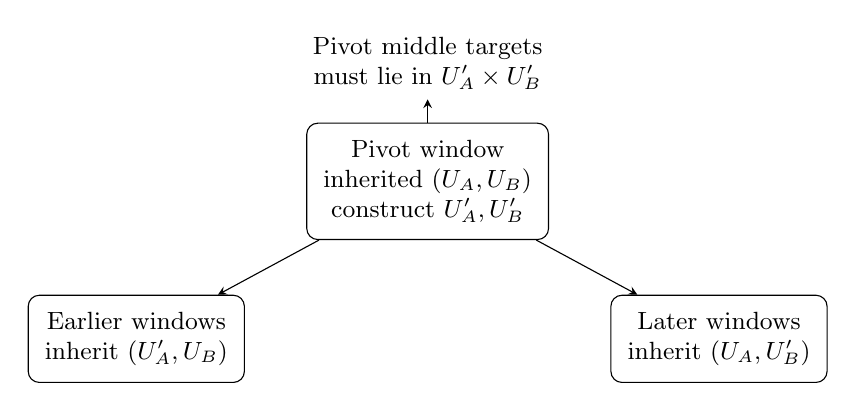
\begin{tikzpicture}[>=stealth,
 every node/.style={align=center,font=\small},
 box/.style={draw,rounded corners,inner sep=6pt}]
 \node[box] (pivot) at (0,0)
 {Pivot window\\inherited $(U_A,U_B)$\\construct $U_A',U_B'$};
 \node[box] (left) at (-3.7,-2)
 {Earlier windows\\inherit $(U_A',U_B)$};
 \node[box] (right) at (3.7,-2)
 {Later windows\\inherit $(U_A,U_B')$};
 \node (targets) at (0,1.5)
 {Pivot middle targets\\must lie in $U_A'\times U_B'$};
 \draw[->] (pivot) -- (left);
 \draw[->] (pivot) -- (right);
 \draw[->] (pivot) -- (targets);
\end{tikzpicture}
\caption{Only the endpoint facing a pivot's representative is restricted
in each descendant half.  All tests are constructed before checking
which actual middle targets they retain.}
\label{fig:pivot-tree}
\end{figure}

At a node, trim $A$ and $B$ to their inherited sets.  Drop its entire subtree
if either trim keeps fewer than $.9$ of its original support, or if the
untrimmed same-node density exceeds $\sigma^{-1000\beta}/q$.
Otherwise, the trimmed supports satisfy Theorem~\ref{thm:predictor} in
dimension four, with $b=O(K_*)$.  Apply the predictor in the orientation
of the smaller support and then Lemma~\ref{lem:fresh-test}, exchanging
the two systems if necessary.  Drop the subtree on failure.  Use
independent tables for each tree address, stage, predictor call and
validation test.

\begin{lemma}[Tree retention]\label{lem:pivot-retention}
The expected number of windows lost by this construction and the
preceding deletions is $o(w)$, where $w$ is the deterministic window
count before deletions.  Among the middle targets, the expected number
lost beyond their fixed non-middle complement is $o(k)$.
Consequently, with probability bounded below, a deterministic
$\Theta(k)$ middle targets can be retained, in order, in the two caps
of their successful pivots.
\end{lemma}

\begin{proof}
Do not inspect actual middle-target coverage while constructing the
tree.  Conditional on history, fresh representative indices and all
original support choices, apply~\eqref{eq:fresh-test-domination} to
each produced ancestor test.  Its hidden source is always a constant
fraction of the original support $X$: the node trim keeps $.9$, the
predictor captures a constant fraction, and the first validation keeps
$.9$ of the opposite trimmed support.  Predictor bias therefore does
not affect this bound.
The readiness indicator has already been removed on the right-hand side
of~\eqref{eq:fresh-test-domination}.  We may therefore sum that bound
over a descendant's original support before averaging its level choice;
we never replace that support by its law conditional on reaching the
descendant.

Average the bound over the independently chosen levels.  For every
descendant's original support, the expected fraction evicted by a
relevant ancestor fresh test is $O(\sigma^{-2000\beta})$ by
\eqref{eq:low-conflict} and Lemma~\ref{lem:flat-levels}.
Inherited sets are intersections of precisely these ambient tests.
The probability of reaching a node but failing its $.9$ trim is thus
at most a constant times the sum of these loss bounds along its path.
The same-node density rejection probability, even ignoring reach, is
$O(\sigma^{-1000\beta})$ by Markov.  Predictor and validation failures
contribute $O(e^{-cq})$ per attempted node.

The tree depth is $O(\log(w+1))=O(\log\sigma)$.
For each fixed node, summing failure bounds over its ancestor path
therefore gives $o(1)$ probability of being lost through a dropped
subtree.  Summing over nodes gives $o(w)$ expected loss.  This adds to
the $o(w)$ representative and open-band deletions already proved.

The identical fresh-test estimate applies to actual good middle targets
after integration against their endpoint marginals.  Given history and
fresh indices, these targets are independent of the auxiliary level
choices and public tables.  An earlier target faces a pivot's second
support, and a later target faces its first support, so all relevant
incidence bounds have the required temporal orientation.  At its own
pivot, the target faces both representatives.  Count bad target indices
and bad endpoints as losses.  Their total is $o(k)$ in expectation,
and the path sum bounds the remaining evictions by $o(k)$ as well.

In this argument the first pivot test is counted whenever it is
produced, without conditioning on success of the second test.
Likewise no ancestor test is conditioned on descendant survival.
Thus all the conditional-law estimates used above have the form
actually supplied by Lemma~\ref{lem:fresh-test}.
Markov now gives a positive constant probability of retaining at least
$c k$ middle targets.  Keep exactly $\lfloor c k\rfloor$ in their
original order.
\end{proof}

\subsection{The new decoder and its message length}

The encoder transmits the tree size and node statuses, successful node
constructions, and the retained slot count at each node in tree order.
The parameters $q,\eta,D,L,R,P$ and the deterministic stage budgets are
part of the common protocol.  At each successful node the message also
specifies its orientation, trimmed support sizes, row lengths and row
indices, together with the predictor's diagnostics.  These integers
cost $O(\sigma)$ per node apart from the already charged row indices.
No failed construction is transmitted.  Starting with the two ambient
point systems, the decoder reconstructs every successful ancestor's
caps and therefore the inherited sets for each successful child.
The predictor's message supplies its set $W$; row sizes and row indices
supply the two validation tests.  A proposal row is regenerated using
public uniforms ranked in the decoder's reconstructed finite domain.
The hidden supports determine acceptance, but are not needed to
regenerate an accepted row.  Concatenating the prescribed number
of copies of the pivot domains in the windows' original order specifies
all new slot domains.  The decoder never needs the old context, the old
slot labels, or the identities of the omitted targets.

\begin{lemma}[Cost of the new context]\label{lem:pivot-compression}
The output of Lemma~\ref{lem:pivot-retention} has a new context satisfying
\begin{equation}\label{eq:stage-output}
 \Lambda'\le CqP\log(w+2)(\sigma+wP)+Cw\sigma,
 \qquad \Delta'\le CK_*.
\end{equation}
These are deterministic bounds.  After fixing public tables and
conditioning on retention of the prescribed length, the stream
marginal still has density bounded by a stage constant.
\end{lemma}

\begin{proof}
At a successful pivot let the trimmed sizes be $n_A,n_B$.  Its two caps
have sizes at most $Cq^5/n_B$ and $Cq^5/n_A$.
Their product is at most $Cq^5e^{CK_*}$ by
\eqref{eq:pivot-support-input}.  Incidence mixing bounds the number of
flags in their product by $Cq^4e^{CK_*}$, proving the domain bound.

To sum metadata, define at a node
\[
 G=\log(|U_A||U_B|/q^5),\quad
 b_v=\log(q^5/(n_An_B)),\quad
 d_A=\log(|U_A|/n_A),\quad d_B=\log(|U_B|/n_B).
\]
Then $d_A+d_B=G+b_v$, with $b_v\le CK_*$.
The left child's positive part $G^+$ is at most $d_B+C$, and the
right child's at most $d_A+C$, by the cap size bounds.  Thus the sum
of their positive potentials is at most $G^++CK_*+C$.
The initial potential is $3\sigma+O(1)$.
At every depth the sum of positive potentials over successful nodes is
therefore at most $3\sigma+CwK_*+O(1)$, by accumulating the costs over
their ancestors.  Dropped children only reduce this sum.

The predictor and validations at a successful node cost
$O(qP(d_A+d_B+P))$ by Theorem~\ref{thm:predictor} and
Lemma~\ref{lem:fresh-test}.  Since $K_*=o(P)$, summing the last bound
over the $O(\log(w+2))$ depths gives the first term
in~\eqref{eq:stage-output}.  Tree statuses cost $O(w)$; support sizes,
row lengths and retained counts cost $O(w\sigma)$.  Self-delimiting
integer encodings multiply these bounds by at most an absolute constant.
The maximum message length therefore bounds its entropy by $\Lambda'$.

By Lemma~\ref{lem:pivot-retention}, the joint probability of successful
extraction, over the prior law and the independent public tables, is
bounded below.  Average first over the tables and fix a realization
with extraction probability bounded below under the prior law and the
remaining auxiliary choices.  Only then condition on extraction.
The stream marginal density increases by at most the reciprocal of
this constant.  This proves the final assertion without requiring any
uniform capture distribution from the predictor.
\end{proof}

We can now state the full compression step established by the two
sections.

\begin{proposition}[One compression stage]\label{prop:compression-stage}
Suppose a selected consistent tuple and context satisfy
\eqref{eq:stage-input}--\eqref{eq:stage-range}, with deterministic
$\ell=\Theta(k)$ and bounded stream-marginal density, and suppose the
rectangle-occupancy event of Lemma~\ref{lem:rectangles} holds almost surely.
Then either the high-rank argument contradicts
Lemma~\ref{lem:stream-entropy}, or a constant-probability extraction
produces another such tuple, of deterministic length $\Theta(k)$, and
a new context satisfying~\eqref{eq:stage-output}, where
\begin{equation}\label{eq:window-count}
 w\le C\sigma^{1+\eta/2}/D.
\end{equation}
Its decoder is independent of the old context.
\end{proposition}

\begin{proof}
Apply Lemma~\ref{lem:marking}, select a deterministic class and window
length by constant-probability conditioning, and use
Lemma~\ref{lem:decoupling}.  Lemma~\ref{lem:high-ranks} eliminates the
high classes.  In reciprocal classes, Lemma~\ref{lem:flat-levels} and
the open-band deletion supply~\eqref{eq:pivot-support-input} and its
averaged incidence bounds.  Lemmas~\ref{lem:pivot-retention}
and~\ref{lem:pivot-compression} finish the construction.
For open bands,~\eqref{eq:window-count} follows from
$k/m\asymp\sigma^{1+\eta/2}/D$.  For integer bands,
$w=O(\sigma^{\eta/2})$, which is smaller because $D\le\sigma$.
All losses and density changes are by stage constants.
\end{proof}

\subsection{The finite iteration}

\begin{theorem}[A stream with no long consistent subsequence]
\label{thm:stream}
For every fixed $0<\eta<1/10$ and every sufficiently large prime $q$,
there is a stream of
$N=\lfloor q^4\log q\rfloor$ flags whose ordered flag graph is
$K_5$-free and has independence number less than
$k=\lfloor q(\log q)^{1+\eta}\rfloor$.
\end{theorem}

\begin{proof}
Suppose instead that every stream has a consistent subsequence of
length $k$.  Choose one and condition the stream on the rectangle
occupancy event of Lemma~\ref{lem:rectangles}, whose probability tends
to one.  Lemma~\ref{lem:stream-entropy} applies to it and to every
constant-density extraction considered above.
Initially the context is empty and every domain is the full flag set,
so $\Lambda=0$ and $\Delta=3\sigma+O(1)$.  Thus
\[
 D=O(\sigma^{1-\eta+\beta})\le\sigma^{1-\eta/2}.
\]
We show that the admissible range is preserved while the context shrinks.

For sufficiently large $q$, $P\le3D\sigma^{9\beta}$.
Substituting this and~\eqref{eq:window-count}
into~\eqref{eq:stage-output} gives
\begin{align*}
 \frac{\Lambda'}{k}
 &\le CD\log\sigma
       \bigl(\sigma^{9\beta-\eta}
                +\sigma^{18\beta-\eta/2}\bigr)+o(1)\\
 &\le D\sigma^{-\eta/3},
 \qquad \Delta'\le CD\sigma^{6\beta}.
\end{align*}
Here the term $Cw\sigma/k$ is exponentially small in $\sigma$;
all other inequalities use $\beta=\eta/10^7$.
The next stage parameter consequently satisfies
\begin{equation}\label{eq:D-recurrence}
 D_{\mathrm{new}}
 =\sigma^\beta(1+\Lambda'/k+\Delta'\sigma^{-\eta})
 \le\sigma^{2\beta}+D\sigma^{-\eta/4}.
\end{equation}
This remains in~\eqref{eq:stage-range}.
After $O(1/\eta)$ applications it gives $D\le2\sigma^{2\beta}$.
One more compression therefore yields
\[
 \Lambda'/k=o(1),\qquad
 \Delta' q\sigma/k=O(\sigma^{8\beta-\eta})=o(1).
\]

At this point run just the marking scans.  Encoding the context,
the masks, the expensive flags and then the remaining cheap flags gives
\[
 H(F)\le4\sigma\ell+O(k)+\Lambda'+O(\Delta' q\sigma)
       =4\sigma\ell+O(k).
\]
But Lemma~\ref{lem:stream-entropy} gives
$H(F)\ge4\sigma\ell+\eta\ell\log\sigma-O(k)$.
Since the deterministic retained length is still $\ell=\Theta(k)$,
these estimates contradict each other for sufficiently large $q$.
Only a fixed number of stages, depending on $\eta$, was used, so all
retention fractions and density bounds remain constants.  The original
assumption is false.  The flag graph of the resulting stream is
$K_5$-free by the ordered-flag construction, completing the proof.
\end{proof}

\section{Preparing the sparse-pair description}
\label{sec:predictor-setup}

We now prove Theorem~\ref{thm:predictor}. The proof is by induction
on the projective dimension \(d\). A large concentration on a proper
flat reduces the dimension. Otherwise, a small collection of flats
records all relevant concentrations, and the score in
Section~\ref{sec:predictor-score} gives the required description.

The following consequences of the parameter choices will be used
throughout:
\begin{equation}
\label{eq:parameter-orders}
 P=o(\sigma),\quad \log\sigma=o(P),\quad
 R\log L=o(P),\quad b+P\tau=o(L),\quad L=o(P).
\end{equation}
For example, \(P\le3D\sigma^{9\beta}\), whereas
\(D\le\sigma^{1-\eta/2}\); also \(b/L=O(\sigma^{-2\beta})\)
and \(P\tau/L=R\tau=o(1)\).
In particular, all fixed numerical constants used below are
eventually smaller than \(R\).

\subsection{Small sets and greedy removal of flats}

Orient the input so that \(n=|S|\le|T|\), and put \(n=q^{1+v}\).
Lemma~\ref{lem:incidence} gives \(n\le Cq^{(d+1)/2}\).
If \(n\le100qP\), send \(n\) and the rank of \(S\) among the
\(n\)-element subsets of the known set \(U_S\).
The elementary inequality
\(\binom{|U_S|}{n}\le(e|U_S|/n)^n\) bounds the message length by
\[
 O\bigl(\sigma+n(d_S+1)\bigr)
 \le CqP(d_S+P).
\]
The decoder takes \(W=S\). Henceforth \(n>100qP\), so \(v>0\).

Define
\[
 g_0=(v-\tfrac12)\sigma,\qquad g_1=(v-1)\sigma,\qquad
 \xi=L/100,\qquad \chi=P/100,\qquad \chi_0=P/10000.
\]
The following two greedy procedures refer to the original value
of \(n\), including in their thresholds.

\begin{enumerate}
\item If \(d=4\) and \(g_1>\chi_0\), repeatedly choose a hyperplane
containing the largest number of remaining points of \(S\).
Remove its remaining points whenever this number is at least \(q^2\).
Stop as soon as at least \(n/2\) points have been removed, or when
the maximum is below \(q^2\).
In the first case retain the removed points and their ordered list
of hyperplanes. In the second retain the residual and no list.
If the procedure is not used, retain all of \(S\).
Call the retained set \(S_1\).
\item If \(d\ge3\) and \(g_0>\chi_0\), apply the same rule to planes
and the points of \(S_1\), now with threshold
\[
 K_p=n^{4/3}q^{-1}\exp(-g_0/5).
\]
Stop on removing at least \(|S_1|/2\), or when the largest
remaining plane count is below \(K_p\).
Retain the removed points and the ordered plane list in the first
case, and the residual with no plane list in the second.
If this procedure is not used, retain \(S_1\).
Write \(S'\) for the final training set and \(n'=|S'|\).
\end{enumerate}

Ties are resolved by a fixed ordering of flats. Each retained list
partitions the training points by \emph{earliest membership}:
a point belongs to the first listed flat containing it. The
hyperplane partition, if present, is restricted to \(S'\) after
the second procedure. The sizes of the original hyperplane
cells, before that restriction, will also be used in the
geometric analysis; they are not needed by the decoder.

\begin{lemma}[Training data]
\label{lem:training}
The construction has \(n/4\le n'\le n\).
If the hyperplane list or plane list is present, its length satisfies
\[
 J_h\le n/q^2,\qquad
 J_p\le n/K_p=q^{1/2}\exp(-2g_0/15),
\]
respectively. If both lists are present, then
\(J_hJ_p\le q^{13/15+o(1)}\).
If a performed procedure retained a residual, that residual has
the corresponding flat cap.

If every training cell in both partitions has size less than
\(.04n'\), then for each query point \(x\) define \(O_x\) as the
union of the following cells: the cell of the earliest listed
hyperplane containing \(x\), and the cell of the earliest listed
plane containing \(x\). Omit a cell when no such flat exists.
Then \(|O_x|/n'<.08\). We call this the \emph{small-cell case}.

The ordered lists, \(n'\), all training cell sizes, and the table
of intersections between the two partitions can be communicated
in \(O(q)\) bits. From these data the decoder determines
\(|O_x|/n'\) for every \(x\), and determines which samples belong
to \(O_x\) from their flat memberships.
\end{lemma}

\begin{proof}
Every retention keeps at least half the previous set.
Each listed flat removes at least its threshold, and its assigned
points are disjoint from those of earlier flats, proving the
length bounds. In dimension four,
\[
 J_hJ_p
 \le q^{v-1}q^{1/2-(2/15)(v-1/2)}
 =q^{13v/15-13/30}
 \le q^{13/15+o(1)},
\]
because \(v\le3/2+O(1/\sigma)\).
Each single list has length at most \(q^{1/2+o(1)}\).
A flat is described by a basis in a fixed coordinate system, using
\(O(\sigma)\) bits; every cell or intersection size uses
\(O(\sigma)\) bits as well. These bounds give \(O(q)\) in total.
The union formula and the intersection table give \(|O_x|\).
For a sampled point, earliest membership in a known list determines
its cell. Finally the union involves at most two cells of size
less than \(.04n'\).
\end{proof}

\subsection{A large cell reduces the dimension}

Suppose a training cell has at least \(.04n'\) points.
Its listed flat \(K_0\), of projective dimension \(2\le j<d\),
satisfies
\[
 S_0=S\cap K_0,\qquad |S_0|\ge .01n.
\]
The encoder sends \(K_0\), with a canonical coordinate system.
The average incidence proportion from \(T\) into \(S_0\) is at
most \(100\tau/q\). Delete members whose proportion exceeds
\(\sqrt\tau/q\). This loses at most \(100\sqrt\tau\,|T|\) members,
so leaves at least \(|T|/2\) for large \(q\).
Each remaining covector restricts nontrivially to \(K_0\).

Normalize each nonzero projective restriction. Each restriction
has at most \(q^{d-j}\) projective lifts: after fixing one
nonzero restricted coordinate to be \(1\), the remaining \(d-j\)
coordinates are free. Among the dyads \([l,2l)\) of lift
multiplicity, choose one carrying at least \(|T|/(C\sigma)\)
of the retained lift mass. Let \(T_0\) be its set of distinct
restrictions. Then
\begin{equation}
\label{eq:reduced-pair}
 |S_0||T_0|\ge q^{j+1}\exp\{-b-O(\log\sigma)\},
 \qquad
 \frac{e(S_0,T_0)}{|S_0||T_0|}\le\frac{\sqrt\tau}{q}.
\end{equation}
Indeed, the number of restrictions is at least the retained mass
divided by \(2l\), and \(l\le q^{d-j}\).
The density assertion holds for each restriction separately,
so forgetting its multiplicity causes no problem.

The decoder's enclosures are
\[
 U_{S_0}=U_S\cap K_0,\qquad
 U_{T_0}=\{\text{nonzero projective restrictions with at least \(l\) lifts in \(U_T\)}\}.
\]
Their logarithmic gaps are bounded by
\(d_S+O(1)\) and \(d_T+O(\log\sigma)\).
The extra term in \(b\) in \eqref{eq:reduced-pair} is absorbed in
\(O(D\sigma^{6\beta})\). Moreover,
\[
 \sqrt\tau\le
 \sigma^{-200\cdot2^{j-2}\beta}\qquad(j<d).
\]
Thus the induction hypothesis applies after orienting the reduced
pair so that its smaller side is first. The dimension decreases,
and its initial value is at most four.

If the recursive output captures \(S_0\), it already captures
a constant fraction of \(S\) in a set of size at most \(ne^{CP}\).
Intersect it with \(U_S\), if necessary.
If instead it captures \(T_0\), let \(W_0\) be the decoded set and
\(C_0=W_0\cap T_0\) its hidden capture, with
\(|C_0|\ge c|T_0|\) and \(|W_0|/|C_0|\le e^{CP}\).
We convert this to a capture on the original side.

Take \(h=\lceil Cq(d_S+1)\rceil\) independent uniform samples
from \(C_0\), temporarily using the true hidden-set law.
On \(U_S\cap K_0\) define the cap
\[
 W=\{x:\text{fewer than } .2h/q
       \text{ of the sampled restrictions annihilate }x\}.
\]
By Lemma~\ref{lem:incidence}, at most \(C'q^{j+1}/|T_0|\)
points in the whole \(j\)-space have incidence proportion
less than \(.5/q\) into \(C_0\).
Every other point belongs to \(W\) with probability at most
\(\exp(-ch/q)\).
The bounds
\[
 |U_S\cap K_0|\le e^{d_S}n,\qquad
 n\le Cq^{j+1}/|T_0|
\]
therefore imply, by increasing \(C\) and applying Markov's
inequality, that
\[
 |W|\le C''q^{j+1}/|T_0|
 \le n\exp\{O(b+\log\sigma+1)\}
\]
with probability at least \(.9\).
The second displayed inequality for \(n\) follows by applying
mixing to \(S_0,T_0\) and using \(|S_0|\ge .01n\).

Every member of \(T_0\) has incidence proportion at most
\(\sqrt\tau/q\) into \(S_0\). Consequently every all-in-\(C_0\)
sample row, regardless of its bias, loses at most
\(5\sqrt\tau\,|S_0|\) points of \(S_0\) under this test:
sum the hit counts and divide by the rejection threshold.
Thus a row satisfying the size test also captures at least
\(.9|S_0|\) for large \(q\).

To implement this sampling with a message, send the integer \(h\)
and use a fresh table indexed by this row length.
Its \(O(\sigma)\)-bit cost is absorbed in the bounds below.
Propose independent rows uniform in the known \(W_0\).
A row falls entirely in \(C_0\)
and passes the size test with probability at least
\(.9e^{-ChP}\). Searching at most \(\exp(C'hP)\) rows gives
failure probability \(O(e^{-cq})\), and its row index takes
\(O(hP)\) bits. Conditional on being all in \(C_0\), a proposed
row is exactly iid uniform in \(C_0\); the comparison is made
before searching. After search, no unbiased-sampling assertion
is used.

The flat, dyad, recursive message, row length and optional conversion
have total length \(O(qP(d_S+d_T+P))\).
Here the recursive increases of \(O(\log\sigma)\) in the gaps
are absorbed because \(\log\sigma=o(P)\).
There are at most two dimension reductions, and each uses
fresh tables. The constants and failure probabilities can
therefore be absorbed in those of Theorem~\ref{thm:predictor}.

We have reduced the proof to training data satisfying the small-cell
case of Lemma~\ref{lem:training}. The next section bounds the rich
radial configurations that can correlate incidence tests at one
query point. Those bounds will be applied separately to validation
on \(S'\) and to output size in the ambient space.

\section{Rich lines and overlapping hyperplanes}\label{sec:geometry}

The score used by the predictor is a sum over hyperplanes through a query
point.  Its terms can depend strongly on one another when two hyperplanes
contain many common training points.  We now bound these overlaps.  The
training-set construction in Lemma~\ref{lem:training} removes large flat
concentrations from each query's samples; the remaining concentrations are
controlled by a polynomial argument for lines and a counting argument for
planes.

Low-degree polynomials vanishing on point sets play a central role in
Dvir's finite-field Kakeya argument \cite{Dvir2009}.
The rich-line proof here uses the polynomial interpolation and tangent-plane
methods of Guth and Katz~\cite{GuthKatz2010} and Elekes, Kaplan, and
Sharir~\cite{ElekesKaplanSharir2011}.  The positive-characteristic
obstruction to these methods is treated by Ellenberg and
Hablicsek~\cite{EllenbergHablicsek2016}.  Here the defining polynomial
has degree below the prime characteristic, and we give the required
algebraic argument in full.
Koll\'ar's positive-characteristic incidence estimate
\cite[Theorem~2]{Kollar} also motivated the rich-line framework. The
plane-capped estimate below is proved directly and does not invoke that
theorem as a premise.

Throughout this section, $q$ is a sufficiently large prime,
$\sigma=\log q$, $\log\sigma=o(P)$ and $P=o(\sigma)$.  Write
\[
 \begin{gathered}
 n=q^{1+v},\qquad \frac n4\le n'\le n,\qquad
 g_0=(v-\tfrac12)\sigma,\qquad g_1=(v-1)\sigma,\\
 \chi=\frac P{100},\qquad \chi_0=\frac P{10000}.
 \end{gathered}
\]
All constants below are absolute.  Bounds denoted by $o(n)$ are uniform
under the parameter assumptions just stated and those of the relevant
lemma.

\subsection{A polynomial bound for rich lines}

We first prove the only algebraic ingredient.  Its characteristic
restriction will enter through a polynomial whose degree is less than $q$.

\begin{lemma}[Rich lines with a plane cap]\label{lem:rich-lines}
Suppose $n=q^{1+v}$, $v\le 3/2+O(1/\sigma)$,
$n/4\le n'\le n$, $g_0>\chi_0$, and
$e^{-g_0/20}<a\le2$.  Put
\[
 M=\frac{n'a}{q},\qquad
 K=n^{4/3}q^{-1}e^{-g_0/5}.
\]
Let $X$ be a set of at most $n$ points of $\mathrm{PG}(d,q)$, where
$3\le d\le4$, such that every projective plane contains at most $K$
points of $X$.  The number of lines containing at least $M$ points of $X$
is at most $Cn/M$.
\end{lemma}

\begin{proof}
The inequalities that make the argument work are
\begin{equation}\label{eq:rich-line-parameters}
 \frac{M}{n^{1/3}}\ge c e^{37g_0/60},\qquad
 \frac{M^2}{K}\ge c e^{23g_0/30},\qquad
 cq\le\frac nM\le Cq e^{g_0/20}.
\end{equation}
They follow by substituting $v=1/2+g_0/\sigma$ and using
$a>e^{-g_0/20}$ and $n'\ge n/4$.  In particular, their first two
ratios tend to infinity.

Work temporarily over an algebraic closure of $\mathbb F_q$.  A generic
linear map to a four-dimensional vector space preserves the independence
of every independent subset of at most four points of $X$.  Indeed, each
of these finitely many requirements defines a nonempty open condition on
the map, and the field is infinite.  The resulting projection to
projective three-space preserves distinct points and distinct rich lines.
It also preserves the plane cap: four projected points in a plane cannot
have come from four independent points.  Choose an affine chart containing
all projected points.

Sample these points independently with probability
\[
 f=A\frac{\sqrt n}{M^{3/2}},
\]
where $A$ is a sufficiently large fixed constant.  By
\eqref{eq:rich-line-parameters}, $f=o(1)$ and
$fM=A\sqrt{n/M}\ge cA\sqrt q$.  There are at most $n^2$ lines containing
at least two points of $X$.  Chernoff's inequality and a union bound imply
that, with probability $1-o(1)$, every rich line contains more than $fM/2$
sampled points.  Markov's inequality gives probability at least $1/2$ that
the total sample size is at most $2fn$.  Choose a sample satisfying both
conditions.

Counting monomials in three variables produces a nonzero polynomial
vanishing on that sample, of degree
\[
 D_0\le C A^{1/3}\sqrt{n/M}.
\]
For sufficiently large fixed $A$, this degree is less than $fM/2$, so the
polynomial vanishes identically on every rich line.  Replacing it by its
squarefree part does not increase the degree or lose any such line.  Also
\begin{equation}\label{eq:degree-characteristic}
 D_0=o(M),\qquad D_0=O(q^{21/40})<q,
\end{equation}
because $g_0\le\sigma+O(1)$.

First consider its plane factors.  At most $D_0^2$ lines lie in two
different factor planes.  Fix one factor plane containing $r$ of the
remaining lines, and choose $M'=\lfloor M\rfloor$ points on each line.
If $d_z$ is their multiplicity at a selected point, the plane cap and the
fact that two lines meet at most once give
\[
 (rM')^2\le K\sum_z d_z^2
 \le K\bigl(rM'+r(r-1)\bigr).
\]
Consequently $r\le KM'/((M')^2-K)=o(M')$.  Delete from each line its
intersections with all other factor planes, removing at most $D_0$ points.
The remaining union in this plane has size at least
\[
 r(M'-D_0)-\binom r2\ge \frac{rM'}2.
\]
These unions are disjoint for different factor planes.  They account for
at most $Cn/M$ lines in total.

Let $F_0$ be the squarefree product of the nonplane factors, and consider
the remaining rich lines.  Call a point of $X$ busy if it lies on at least
three of these lines.  At a busy point where $\nabla F_0\ne0$, the three
distinct line directions lie in the tangent plane, and the Hessian
quadratic form vanishes on them.  A quadratic form on a two-dimensional
space with three distinct projective zeros is identically zero.  Since
the characteristic is odd, polarization shows that the Hessian bilinear
form vanishes on that tangent plane.  Thus every busy point is a zero of
all the polynomials
\begin{equation}\label{eq:hessian-polynomials}
 Q_{ij}=(e_i\mathbin\times\nabla F_0)^t
              \operatorname{Hess}(F_0)
              (e_j\mathbin\times\nabla F_0),\qquad 1\le i,j\le3.
\end{equation}
This is also true at a point with zero gradient.  There are at most $2n$
nonbusy point--line incidences.  Except for $Cn/M$ lines, every remaining
line therefore has at least $M'/2$ busy points.  As $\deg Q_{ij}<3D_0$ and
$M'/2>3D_0$ for large $q$, each such line lies in every $Q_{ij}$.

We claim that no irreducible factor $F$ of $F_0$ divides all the
$Q_{ij}$.  Since $\deg F<q$, some derivative of $F$, say $F_z$, is
nonzero.  Squarefreeness implies that $F$ and $(F_0)_z$ are coprime in
$\overline{\mathbb F}_q(x,y)[z]$.  Clearing a B\'ezout identity in that
field and specializing $x,y$ away from its denominators and the leading
coefficient of $F$ produces a point on $F$ where $(F_0)_z\ne0$.
After translation, the formal implicit-function theorem writes the
surface locally as $z=h(x,y)$.

If every $Q_{ij}$ vanished on this surface, the Hessian bilinear form of
$F_0$ would vanish on its tangent space: the vectors
$e_i\mathbin\times\nabla F_0$ span that space.  Differentiating
$F_0(x,y,h(x,y))=0$ twice would then give
\[
 h_{xx}=h_{xy}=h_{yy}=0.
\]
For a nonzero monomial $x^u y^w$ of $h$, these identities force
$(u,w)$ modulo the prime $q$ to be one of
$(0,0),(1,0),(0,1)$.  Thus $h$ agrees with its affine-linear part $h_1$
through total degree $q-1$.  The polynomial $F_0(x,y,h_1(x,y))$ has degree
less than $q$ and vanishes to order at least $q$, so it is zero.  This
would give a plane factor of $F_0$, a contradiction.

Over the algebraic closure, a constant linear combination $Q$ of the
$Q_{ij}$ can therefore be chosen coprime to $F_0$: avoid the finitely many
proper linear subspaces of coefficients corresponding to its irreducible
factors.  We use the following elementary consequence of resultants.
\begin{quote}
Two coprime polynomials in affine three-space, of degrees $D_1,D_2$,
contain at most $2D_1D_2$ common lines.
\end{quote}
Here is a proof sufficient for this application.  Choose a linear
coordinate $z$ nonconstant on every line in any fixed finite collection
of common lines.  For a generic value $s$, the restrictions to $z=s$
remain nonzero and coprime.  To see this, use the nonzero resultants
eliminating $y$ and eliminating $x$, viewed over the respective fraction
fields; preserve a nonzero coefficient of each applicable resultant
under specialization.  A common factor of positive degree in either
variable would make the corresponding resultant vanish.  If both
polynomials are independent of an elimination variable, omit that
resultant.  Nonvanishing of the specialized polynomials is a further
open condition.  This argument remains valid when degrees drop: a common
factor supplies a kernel vector for the Sylvester map within the original
degree bounds.

Avoid also the finitely many values $s$ at intersections of selected
lines.  Their slice points are distinct.  Choose coordinates in the slice
so their first coordinates are distinct.  The resultant eliminating the
second coordinate is nonzero, has degree at most $2D_1D_2$, and vanishes
at each of those first coordinates.  If both polynomials are independent
of the second coordinate, coprimality gives no common point instead.
This proves the assertion.  Applied to $F_0,Q$, it bounds the remaining
lines by $O(D_0^2)=O(n/M)$, completing the proof.
\end{proof}

\subsection{The overlap estimate}

We now return to the training set.  To keep the geometric statement
independent of the score, the hyperplanes below can be any family of
bounded training density.

\begin{lemma}[Geometry of the training set]\label{lem:overlap-geometry}
Let $3\le d\le4$, $100qP<n=q^{1+v}\le Cq^{(d+1)/2}$, and let
$S'\subset\mathrm{PG}(d,q)$ be the training set in the small-cell case of
Lemma~\ref{lem:training}, with $n'=|S'|\in[n/4,n]$.
For each query point $x$, let $O_x$ be the union of its earliest containing
assignment cells in the captured hyperplane and plane lists; an absent
list contributes the empty set.  Put
\[
 X_x=S'\setminus(O_x\cup\{x\}),\qquad B=\frac{q^d}{n'},\qquad
 a_\ell=\frac{q|X_x\cap\ell|}{n'}
\]
for lines $\ell$ through $x$.
For each $x$, let $\mathcal H_x$ be any family of hyperplanes through $x$
such that $q|X_x\cap H|/n'\le2$ for every $H\in\mathcal H_x$.
For distinct members set
\[
 \theta_{HH'}=\frac{q|X_x\cap H\cap H'|}{n'},
\]
and let $E_x(a)$ count ordered distinct pairs with $\theta_{HH'}\ge a$.
Let $\Delta_x(a)$ be the maximum degree of this relation.

There is a set of $o(n)$ query points outside which, simultaneously for
all dyadic $a\in[q^{-10},2]$,
\begin{align}
 \#\{\ell\ni x:a_\ell\ge a\}
   &\le q^{2-2v}e^\chi a^{-100},\label{eq:local-rich-lines}\\
 E_x(a)&\le B^2e^{2\chi}a^{-200},\label{eq:overlap-pairs}\\
 \Delta_x(a)&\le Be^{2\chi}a^{-200}.\label{eq:overlap-degree}
\end{align}
The exceptional set is independent of the choice of the families
$\mathcal H_x$.

Let $p$ be an even integer in
$[10000\sigma/P,10000\sigma/P+2]$ and put $t=1/(100p)$.
After excluding at most $n\exp(CP)$ additional points,
\begin{equation}\label{eq:ambient-overlap-degree}
 \Delta_x(t)\le B e^{-3P}.
\end{equation}
These additional points are needed only for the ambient bound, and are
not included in the $o(n)$ validation exception.

Two further estimates hold without point exclusions.  Every line strength
is at most $Ce^{-g_1}$.  If $g_0>\chi_0$ and
$e^{-g_0/20}<a\le2$, the number of pairs $(x,\ell)$ with $x\in\ell$ and
$a_\ell\ge a$ is at most $Cq^2/a^2$.  For all strengths, the number of
possible point--line pairs is at most $Cq^7$.
\end{lemma}

\begin{proof}
We first prove the line estimates.  Since the radial lines partition
$X_x$, their number of strength at least $a$ is at most $q/a$.  This
implies \eqref{eq:local-rich-lines} if $g_0\le\chi_0$ or
$a\le e^{-g_0/20}$, because the ratio of the former bound to the latter
is
\[
 e^{2g_0-\chi}a^{99}=o(1).
\]
Suppose otherwise, and put $M=n'a/q$.  The plane-peeling step was then
performed, with threshold
$K_p=n^{4/3}q^{-1}e^{-g_0/5}$ and list length
$J_p\le n/K_p$.  In addition to
\eqref{eq:rich-line-parameters}, we have
\begin{equation}\label{eq:plane-list-length}
 J_p\le q^{1/2}e^{-2g_0/15},\qquad J_p/M\le C e^{-13g_0/12}=o(1).
\end{equation}

If the capped residual was retained, Lemma~\ref{lem:rich-lines} gives
$Cn/M\le Cq/a$ rich lines.  Each has $q+1$ rational centers, so there
are at most $Cq^2/a^2$ relevant center--line pairs.

If a captured prefix of planes was retained, a line not contained in any
listed plane has at most $J_p=o(M)$ training points.  On a line first
contained in plane $j$, earlier planes contribute at most $J_p$ points,
and later assignment cells contribute none.  Cell $j$ must therefore
contribute at least $M/2$ points.  For these points to survive the removal
of $O_x$, the center $x$ must belong to an earlier listed plane.  None of
those earlier planes contains the line, so at most $j$ centers qualify.
Write $f_j$ for the fraction of $S'$ in cell $j$.

If $a>Cf_j$, the incidence variance in that projective plane gives at
most $Cq^{2-v}f_j/a^2$ rich lines in it.  Multiplying by $j$ and summing
uses $\sum_j f_j\le1$ and $J_pq^{2-v}\le q^2$, giving $Cq^2/a^2$
center--line pairs.  If $a\le Cf_j$, the nonincreasing cell sizes from
the greedy plane peel imply $j\le C/a$.  There are at most $Cq^2$ lines
in each such plane, and summing the center multiplicities $j$ again gives
$Cq^2/a^2$.  Additional removal of a hyperplane cell can only decrease
these counts.

We have proved the asserted global center--line bound.  Markov's
inequality at the threshold in \eqref{eq:local-rich-lines} leaves a
fraction at most
\begin{equation}\label{eq:line-exception-fraction}
 C e^{g_1-\chi}a^{98}
\end{equation}
of $n$ exceptional centers.  If $g_1\le\chi_0$, this tends to zero even
after summing over $O(\sigma)$ dyads.  Otherwise every line has strength
at most $q(q+1)/n'\le Ce^{-g_1}$, so the same sum is still smaller.
The crude $Cq^7$ bound counts all points and all lines through them in
projective four-space; it also covers dimension three.

This proves the radial-line bounds. We next estimate the overlap edge
count $E_x(a)$ and maximum degree $\Delta_x(a)$.
Set $M=n'a/q$ for every strength
threshold $a$, including those covered by the trivial line bound.
In dimension three the intersection of two distinct hyperplanes through
$x$ is a radial line.  Each such line gives at most $Cq^2$ ordered pairs.
A fixed $H\in\mathcal H_x$ contains at most $2/a$ radial lines of
strength at least $a$, and each lies in at most $Cq$ other hyperplanes.
Hence
\[
 E_x(a)\le Cq^2\#\{\ell\ni x:a_\ell\ge a\},\qquad
 \Delta_x(a)\le Cq/a.
\]
Because $B\asymp q^{2-v}$ and $v\le1+O(1/\sigma)$, these prove
\eqref{eq:overlap-pairs} and \eqref{eq:overlap-degree} in dimension three.

It remains to analyze dimension four.  Intersections are now planes
through $x$.  Call an overlap plane dominant if one radial line carries
at least half its outside-own points, and nondominant otherwise.  A
dominant overlap of strength at least $a$ contains a line of strength at
least $a/2$.  Each such line gives at most $Cq^4$ ordered hyperplane pairs.
For a fixed $H\in\mathcal H_x$, the corresponding degree is at
most $Cq^2/a$.  Dividing this degree by $B\asymp q^{3-v}$ gives
$Ce^{g_1}/a$.  If $g_1\le\chi_0$, this meets
\eqref{eq:overlap-degree}; if $g_1>\chi_0$, a dominant overlap requires
$a\le Ce^{-g_1}$, and the same ratio is at most $C/a^2$.
Equation~\eqref{eq:local-rich-lines} also gives the required pair count.

In a nondominant plane of strength at least $a$, there are at least
$cM^2$ pairs of training points on distinct radial lines.  Each pair
together with $x$ determines the plane.  Thus the number of these planes
through $x$ is at most $Cq^2/a^2$.  Within a fixed $H\in\mathcal H_x$,
it is at most $C/a^2$, since $|X_x\cap H|\le2n'/q$.
Every plane lies in at most $Cq$ hyperplanes, so
\begin{equation}\label{eq:nondominant-crude}
 E_x(a)\le Cq^4/a^2,\qquad \Delta_x(a)\le Cq/a^2.
\end{equation}
The degree bound is always sufficient.  The pair bound is sufficient if
$g_1\le\chi_0$ or $a\le e^{-g_1/10}$: after dividing by $B^2$, its
extra factor is $Ce^{2g_1}/a^2$, which is then absorbed by
$e^{2\chi}a^{-200}$.

\paragraph{Rich planes in the remaining range.}
Suppose $g_1>\chi_0$ and $a>e^{-g_1/10}$.  Here
\begin{equation}\label{eq:rich-plane-parameters}
 M\gg q,\qquad M^2\gg n.
\end{equation}
If a captured hyperplane list was retained, take as its head the prefix
whose original cell sizes, before plane peeling, exceed $C_0q^2/a$,
where $C_0$ is a sufficiently large absolute constant.  Its length is at
most $na/(C_0q^2)$.  The remaining training tail has hyperplane cap
$C_0q^2/a$, by the maximal choice at every greedy step.  If instead the
hyperplane-capped residual was retained, use an empty head and the whole
training set as tail.

A plane not contained in a head hyperplane receives fewer than $M/4$
head points: each intersection is a line of at most $q+1$ points, and
the displayed head-length bound applies.  Let $\mathcal F$ be the global
family of planes containing at least $M/2$ tail points, and let
\[
 r=|\mathcal F|,\qquad u=q^{4-2v}a^{-3}.
\]
A line is contained in at most $Cn/M=O(u)$ members of $\mathcal F$,
since they are disjoint off that line and $M\gg q$.  A hyperplane is
a projective three-space and has at most $C_0q^2/a$ tail
points.  The incidence variance there bounds the number of its planes in
$\mathcal F$ by
\[
 \frac{Cq^2(C_0q^2/a)}{M^2}=O(u).
\]
The use of variance is valid because the mean is $O(q/a)=o(M)$.

For a query $x$, write $d_x$ for the number of members of $\mathcal F$
through $x$.  In the quotient by $x$ these become lines of a projective
three-space, with at most $Cu$ in any point or plane.  If $d_x>C'u$, a
constant fraction of pairs of these quotient lines are skew.  Indeed,
if no line meets half the others, this is immediate.  Otherwise fix a
line meeting at least half.  Among its neighbors, a given line has only
$O(u)$ companions with the same intersection point or the same spanning
plane with the fixed line.  All remaining pairs of neighbors are skew.
Two corresponding original planes intersect exactly in $x$.  Therefore
\begin{equation}\label{eq:rich-plane-second-moment}
 \sum_{d_x>C'u}d_x^2\le Cr^2.
\end{equation}
Count incidences at the tail points, splitting according to this
threshold and applying Cauchy--Schwarz:
\[
 rM/2\le Cnu+C\sqrt n\,r.
\]
By \eqref{eq:rich-plane-parameters}, $r\le Cnu/M$.  Equation
\eqref{eq:rich-plane-second-moment} now implies that
\begin{equation}\label{eq:rich-plane-local}
 d_x\le q^{4-2v}e^\chi a^{-4}
\end{equation}
outside at most $Cq^2e^{-2\chi}$ centers.

Next consider a rich plane contained in a head hyperplane, and take the
earliest such hyperplane, with index $j$.  Earlier noncontaining cells
contribute fewer than $M/4$ points, and later cells contribute none.
Richness therefore requires at least $M/2$ points of cell $j$.
For these to remain outside $O_x$, the center must lie in an earlier
hyperplane.  This allows at most $Cjq$ centers on the plane.
Let $f_j$ be the original cell size divided by $n$.  If $a>Cf_j$,
variance within hyperplane $j$ bounds these planes by $CBf_j/a^2$.
Summing their center multiplicities gives at most $Cq^3/a$, because
\[
 \sum_j j f_j\le \frac{na}{C_0q^2}\sum_j f_j
 \le\frac{na}{C_0q^2}.
\]
Markov's inequality at the threshold in \eqref{eq:rich-plane-local}
makes the exceptional fraction at most $Cq^{v-2}e^{-\chi}a^3=o(1)$.

If $a\le Cf_j$, then $x$ belongs to two original hyperplanes whose cell
fractions are at least $ca$, by the nonincreasing order.  There are at
most $C/a$ such hyperplanes; the union of their pairwise intersections
has at most $Cq^2/a^2$ points.  Relative to $n$, this is at most
$Ce^{-.8g_1}=o(1)$ in the present range.  All exceptions remain $o(n)$
after summing over the dyads.

We have bounded the number of rich overlap planes through every
remaining $x$ by $Cq^{4-2v}e^\chi a^{-4}$.  Each gives at most $Cq^2$
ordered hyperplane pairs.  This proves
\eqref{eq:overlap-pairs} in the remaining case.  The degree estimate
continues to follow from \eqref{eq:nondominant-crude}.  The fixed powers
of two from neighboring dyads and all constant factors are absorbed by
the exponential slack.  This completes the bounds outside $o(n)$ points.

\paragraph{The stronger bound used only for ambient points.}
If $g_1<-4P$, the dominant-line degree divided by $B$ is at most
$Ce^{g_1}/t\le e^{-3P}$.  If $g_1>\chi_0$, which can occur only in
dimension four, the maximum line strength $Ce^{-g_1}$ is smaller than
$t/2$; there is no dominant strong overlap.

In the remaining range $-4P\le g_1\le\chi_0$, exclude every center with
an outside-own radial line of strength greater than $t/2$.  Here
$g_0=\sigma/2+g_1>\chi_0$ and
$t/2\gg e^{-g_0/20}$, so the global center--line bound already proved
costs at most
\[
 Cq^2/t^2\le n e^{CP}
\]
centers.  There are now no strong pairs in dimension three.  In dimension
four only nondominant strong pairs remain, and
\[
 \Delta_x(t)/B\le Cq^{v-2}t^{-2}
 \le Cq^{-1/2+o(1)}<e^{-3P}.
\]
Here $P=o(\sigma)$ and $\log(1/t)=O(\log\sigma)=o(P)$.
These exclusions give \eqref{eq:ambient-overlap-degree}.  They have not
been charged to the $o(n)$ exceptional set, as required.
\end{proof}

\begin{remark}\label{rem:geometry-validation}
The distinction between the two exceptional sets is essential.  The
second-moment validation argument can lose only $o(n)$ training points,
so it uses \eqref{eq:local-rich-lines}--\eqref{eq:overlap-degree}.
The stronger degree estimate \eqref{eq:ambient-overlap-degree} is used
only to bound the size of the predictor's ambient output, where an
additional $n\exp(CP)$ points are permitted.
\end{remark}

\section{The Poisson score}
\label{sec:predictor-score}

We now construct the set promised by the predictor in the small-cell case.
The training set and its assignment cells come from Lemma~\ref{lem:training}.
The geometric estimates control dependence between tests through the same
query point.  Our immediate task is to turn those estimates into a score
which accepts many training points and few ambient points.

Throughout this section write
\begin{gather*}
 n=|S|=q^{1+v},\qquad n'=|S'|\in[n/4,n],\qquad B=q^d/n',\\
 \xi=L/100,\qquad \chi=P/100,\qquad \chi_0=P/10000.
\end{gather*}
We are in the case \(n>100qP\); the enumeration case was treated earlier.
For a query point \(x\), let \(O_x\subseteq S'\) be its own set: the union
of the assignment cells of the earliest flats containing \(x\) in the two
captured lists.  An absent list contributes the empty set.  Its fraction
\(f=|O_x|/n'\) is at most \(.08\).  The cell table determines this fraction,
including the intersection of the two cells.  It also determines whether a
sampled training point belongs to \(O_x\).

Let \(\mathscr C\) contain the cells from each list and their cross
intersections.  These are three partition systems, so
\(\sum_{C\in\mathscr C}|C|/n'\le3\).  For a hyperplane \(H\), put
\[
 \lambda_H=\frac{q|S'\cap H|}{n'},\qquad
 f_C=\frac{|C|}{n'},\qquad
 \lambda_{H,C}=\frac{q|C\cap H|}{n'}.
\]
The exceptional hyperplanes form the deterministic set
\begin{equation}
 \mathcal E=\{H:|\lambda_H-1|>.1\}
 \ \cup\!\bigcup_{C\in\mathscr C}
       \{H:|\lambda_{H,C}-f_C|>.02\}.
 \label{eq:exceptional-hyperplanes}
\end{equation}
A hyperplane is \emph{typical} if it does not belong to $\mathcal E$.
The encoder may use this set in analyzing a row; the decoder will not need
it to compute the score.

A \emph{pencil} at $x$ is the family of all hyperplanes containing $x$.
Take $R$ independent Poisson batches, each of mean $Lq$, whose points
are independent and uniform in $S'$.  Let $Z\subseteq\mathcal E$ be the
hyperplanes empty in every batch, put $z=|Z|$, and let $z_x$ count the
members of $Z$ containing $x$.

For each point \(x\), set \(b_0=e^{-L(1-f)}\).  Its score is
\begin{equation}
 A_x=\sum_{H\ni x}\prod_{r=1}^R
 \mathbf1\{\text{batch }r\text{ has no point of }O_x\cap H\}
 \bigl(\mathbf1\{\text{batch }r\text{ has no point of }(S'\setminus O_x)
                                      \cap H\}-b_0\bigr).
 \label{eq:poisson-score}
\end{equation}
The procedure includes every sampled point.  It includes an unsampled
point exactly when \(A_x<.5z/q\).  The samples and cell data determine
\eqref{eq:poisson-score}; only the integer \(z\) is additional information.

The score will approximate $z_x$: empty exceptional hyperplanes give
its main contribution, and centering suppresses typical hyperplanes.
We will show that $z_x$ is small for most training points and large
for most ambient points.

\begin{lemma}[Score procedure]
\label{lem:score-procedure}
Assume the small-cell conclusions of Lemma~\ref{lem:training}
and, when \(d\ge3\), the estimates of
Lemma~\ref{lem:overlap-geometry} for outside-own radial lines and hyperplane
pairs.  Assume also
\[
 |S||T|\ge q^{d+1}e^{-b},\qquad
 \frac{e(S,T)}{|S||T|}\le\frac{\tau}{q},\qquad
 b=O(D\sigma^{6\beta}),
\]
with the predictor's parameter ranges and \(2\le d\le4\).
Take \(R\) independent Poisson batches, each of mean \(Lq\), sampled
uniformly from \(S'\).  From the batches, the transmitted cell data and
one additional integer \(z\), this score procedure computes a set
\(W\) of points on the \(S\)-side.  With probability at least
\(\exp[-C(P\tau+1)]\), the row has at most \(2qP\) samples and satisfies
\[
 |W|\le n e^{CP},\qquad |W\cap S'|\ge c n'.
\]
These are simultaneous assertions under the original Poisson sampling
law.  The procedure does not condition on finding a successful row.
\end{lemma}

Here are the geometric inputs used in dimensions three and four, stated
explicitly to fix the interface.  Apart from \(o(n)\) centers, the number of radial lines
of outside-own strength at least \(a\) is at most
\(q^{2-2v}e^\chi a^{-100}\).  Among any pencil family whose outside-own
mass is at most two, the overlap graph at level \(a\) has ordered edge
count and maximum degree at most
\begin{equation}
 E_a\le B^2e^{2\chi}a^{-200},\qquad
 \Delta_a\le Be^{2\chi}a^{-200}.
 \label{eq:score-geometric-inputs}
\end{equation}
For the ambient analysis, after excluding an additional \(ne^{O(P)}\)
centers, its degree at \(t=1/(100p)\) is at most \(Be^{-3P}\), where \(p\)
is an even integer in \([10000\sigma/P,10000\sigma/P+2]\).
In the case \(g_1=(v-1)\sigma>\chi_0\), which occurs only in dimension
four, outside-own strengths are at most \(Ce^{-g_1}\).  The global number
of center--line incidences of strength at least \(a>e^{-.05g_0}\), where
\(g_0=(v-.5)\sigma\), is at most \(Cq^2/a^2\).
Lemma~\ref{lem:overlap-geometry} proves these statements without sampling.
All dyadic levels below range from \(q^{-10}\) to two.  Every positive
strength or overlap is at least \(q/n'\), so this range includes all
nonzero quantities which occur.

We shall repeatedly use the following consequences of the parameter
hierarchy:
\begin{equation}
 \log\sigma=o(P),\quad R\log L=o(P),\quad
 b+P\tau=o(L),\quad L=o(P),\quad P=o(\sigma).
 \label{eq:score-parameter-slack}
\end{equation}
They hold uniformly in the allowed range of \(D\), for fixed \(\eta>0\)
and sufficiently large \(q\).  In particular \(R/2>200\) and \(R>5000\).

\subsection{Empty exceptional hyperplanes}
\label{subsec:score-exceptional}

The incidence variance identity gives
\begin{equation}
 \sum_H(\lambda_{H,C}-f_C)^2\le CqBf_C,
 \qquad \sum_H(\lambda_H-1)^2\le CqB.
 \label{eq:cell-variance}
\end{equation}
Replacing the exact means by \(f_C\) and one changes only a negligible
term, since \(qp_d=1-1/Q_d\).  Summing the first estimate over the three
partition systems, then using the thresholds in
\eqref{eq:exceptional-hyperplanes}, gives
\begin{equation}
 |\mathcal E|\le CqB,\qquad
 \sum_{H\in\mathcal E}\lambda_H\le CqB.
 \label{eq:exceptional-mass}
\end{equation}
For the second assertion, use Cauchy--Schwarz and the full-set variance
in \eqref{eq:cell-variance}.

We call a pencil regular if it contains at most \(Be^\xi\) members of
\(\mathcal E\), and if the pencil sum of each clipped squared deviation
in \eqref{eq:cell-variance} is at most \(Be^\xi\). Here clipping replaces
a squared deviation $u^2$ by $\min\{1,u^2\}$.  Only \(o(n)\) centers
have an irregular pencil.  Indeed, a clipped weight \(w_H\in[0,1]\) has
\(\sum_Hw_H\le CqBf_C\) and \(\sum_Hw_H^2\le\sum_Hw_H\).  Applying
incidence variance in the opposite direction gives a total pencil
variance at most \(Cq^dBf_C\), with mean \(O(Bf_C)\).  Chebyshev's
inequality bounds its exceptional centers by \(Cn'e^{-2\xi}f_C\).
Sum this bound using \(\sum_Cf_C\le3\); the full-set and exceptional-set
indicator estimates have the same proof.  This argument pays for the
number of cells through their total mass, not their cardinality.

Poisson splitting makes the sample counts at different point--batch
pairs independent.  The average of \(\lambda_H\) over
\(H\in T\) is at most \(4\tau\).  Thus there is a fixed
\(T_0\subseteq T\) with \(|T_0|\ge|T|/2\) and \(\lambda_H\le8\tau\)
for every \(H\in T_0\).  For large \(q\), these hyperplanes lie in
\(\mathcal E\), and the product-size assumption gives
\(|T_0|\ge cqBe^{-b}\).
If \(Y\) counts the members of \(T_0\) empty in all batches, then
\[
 \EE Y\ge |T_0|e^{-8P\tau},\qquad 0\le Y\le |T_0|.
\]
The second bound, rather than independence of empty-hyperplane events,
yields
\begin{equation}
 \PP\{z\ge z_{\min}\}\ge\tfrac12e^{-8P\tau},
 \qquad z_{\min}=cqB e^{-b-8P\tau}.
 \label{eq:z-event}
\end{equation}
Here and below decrease the absolute constant \(c\) if necessary.

We may require at the same time
\begin{equation}
 \sum_{H\in Z}\lambda_H\le .001z.
 \label{eq:z-small-mass}
\end{equation}
The terms with \(\lambda_H\le10^{-4}\) contribute at most \(10^{-4}z\).
For the others, \eqref{eq:exceptional-mass} gives expected contribution
at most \(CqBe^{-10^{-4}P}\).  Markov's inequality at
\(.0009z_{\min}\) fails with probability at most
\(Ce^{b+8P\tau-10^{-4}P}=o(e^{-8P\tau})\), by
\eqref{eq:score-parameter-slack}.

For each resulting \(Z\), incidence variance shows that
\begin{equation}
 z_x\ge .8z/q
 \quad\hbox{outside at most }Cq^{d+1}/z\hbox{ ambient points}.
 \label{eq:z-ambient}
\end{equation}
On the training set,
\[
 \sum_{x\in S'}z_x=\frac{n'}q\sum_{H\in Z}\lambda_H\le .001n'z/q.
\]
Consequently at least \(.99n'\) training points satisfy \(z_x\le .1z/q\).


The exceptional part of the score equals \((1-b_0)^Rz_x\), with error in
absolute value at most \(b_0|\mathcal E\cap\{H:H\ni x\}|\).  For a member
of \(Z\) every factor is \(1-b_0\).  For any other exceptional hyperplane,
either an own hit makes its product zero or an outside-own hit supplies a
factor \(-b_0\); every other factor has magnitude at most one.  At a
regular pencil the error is at most \(Be^{-.91L}=o(z_{\min}/q)\), and
\((1-b_0)^R=1-o(1)\).  It remains to control the sum \(T_x\) over the
nonexceptional hyperplanes.  This is the only probabilistic issue left
in separating the two bounds on \(z_x\).

\subsection{The second moment on training points}
\label{subsec:score-second-moment}

Fix \(x\). The \emph{schedule} of a point or direction is the vector of
its sample counts in the $R$ batches. Condition first on \(x\) being
unsampled and then on the schedules of all points of
\(O_x\setminus\{x\}\).  The own-empty
multipliers in \eqref{eq:poisson-score} are now fixed zeros or ones.
All remaining point counts are still independent Poisson variables.
Group them by their radial lines \(\ell\) through \(x\), with strengths
\[
 a_\ell=\frac q{n'}|\ell\cap(S'\setminus(O_x\cup\{x\}))|.
\]
A line has a hit in a specified batch with probability \(1-e^{-La_\ell}\).
For a typical hyperplane put
\[
 \lambda'_H=\sum_{\ell\subset H}a_\ell,\qquad
 \delta'_H=\lambda'_H-(1-f),\qquad
 \theta_{HH'}=\sum_{\ell\subset H\cap H'}a_\ell.
\]
The union defining \(O_x\) uses two cells minus their intersection.
The exceptional thresholds therefore give
\begin{equation}
 \lambda'_H\ge .75,\qquad |\delta'_H|\le .17,\qquad
 D_x:=\sum_{H\text{ typical}}(\delta'_H)^2\le CBe^\xi
 \label{eq:typical-masses}
\end{equation}
at a regular pencil.  The last bound follows by summing the relevant
clipped squares.  Removing \(x\) contributes at most
\(O(q^{d-1}(q/n')^2)=O(B)\), since \(n'\ge n/4>25qP\).
Also \(\lambda'_H\le\lambda_H\le1.1\), so the geometric input applies.

Temporarily omit the fixed own multiplier and write the one-batch term as
\[
 X_H=\mathbf1\{H\text{ is outside-own empty}\}-b_0.
\]
Then
\[
 u_H:=\EE X_H=e^{-L\lambda'_H}-b_0,
 \qquad |u_H|\le Le^{-.75L}|\delta'_H|,
\]
and for distinct \(H,H'\),
\[
 \EE X_HX_{H'}=u_Hu_{H'}+
 e^{-L(\lambda'_H+\lambda'_{H'})}(e^{L\theta_{HH'}}-1).
\]
Since \(\lambda'_H+\lambda'_{H'}-\theta_{HH'}\ge .75\),
\begin{equation}
 |\EE X_HX_{H'}|\le L^2e^{-.75L}
       (|\delta'_H\delta'_{H'}|+\theta_{HH'}),
 \qquad \EE X_H^2\le2e^{-.75L}.
 \label{eq:one-batch-moments}
\end{equation}
The fixed multipliers can only reduce the absolute bounds.
More precisely, after the own schedules are fixed, the full product
for a hyperplane is either identically zero or has all its own-empty
multipliers equal to one.  Thus they do not alter the signed
cancellation used below.

In dimension two the overlaps vanish.  In higher dimensions,
\eqref{eq:score-geometric-inputs} and dyadic summation give
\[
 \sum_{H\ne H'}\theta_{HH'}^R
 \le B^2\exp(2\chi+O(R+\log\sigma)).
\]
For the deviation terms, \(R\ge2\) and \(|\delta'_H|<1\) give
\(\sum_{H,H'}|\delta'_H\delta'_{H'}|^R\le D_x^2\).
Finally \(Q_{d-1}=O(B^2)\), because
\(n'\le n\le Cq^{(d+1)/2}\).  Summing
\eqref{eq:one-batch-moments} to the \(R\)-th power and using
\eqref{eq:score-parameter-slack} proves
\begin{equation}
 \EE T_x^2\le B^2e^{-.6P}.
 \label{eq:validation-second-moment}
\end{equation}
This estimate is uniform in the conditioned own schedules.  It holds
at all centers except the \(o(n)\) pencil and geometric exceptions;
it uses none of the additional ambient exclusions.

In dimension two, different pencil lines have disjoint outside-\(x\)
samples.  Thus their score terms are independent under the same
conditioning.  Their variance sum is at most \(Cqe^{-.6P}\), and their
mean is at most \(Be^{-cP}\), by the one-batch mean bound and \(D_x\).
Bernstein's inequality gives
\begin{equation}
 \PP\{|T_x|>z_{\min}/(10q)\}\le q^{-50}.
 \label{eq:score-dimension-two}
\end{equation}
Indeed \(B\ge c\sqrt q\), \(P=o(\sigma)\), and \(e^{cP}\gg\sigma\).
This settles the ambient tail in dimension two.  The next subsection
treats dimensions three and four, where pencil tests share radial lines.

\subsection{An ambient moment bound}
\label{subsec:score-high-moment}

Choose the even moment order \(p\) above, and put \(K_c=200\), \(J=5000\).
If \(g_1>\chi_0\), let \(\mathcal G_x\) be the event that every
outside-own radial line hits in fewer than \(J\) batches.  Otherwise
\(\mathcal G_x\) is the whole sample space.  In the high case a line of
strength \(a\) violates the condition with probability at most
\((2Pa)^J\).  The global geometric line bound and the maximum strength
\(Ce^{-g_1}\) give, after summing the dyads above \(e^{-.05g_0}\),
\[
 \sum_x\PP(\mathcal G_x^c)
 \le Cq^2P^J e^{-(J-2)g_1+O(J)+O(\log\sigma)}+o(n)\le n.
\]
For the lower dyads, the elementary bound of \(Cq^7\) center--line pairs
in dimensions at most four contributes at most
\(Cq^7(CPe^{-.05g_0})^J=o(n)\); here \(g_0>.5\sigma\).
These are probabilities under the fixed-point conditioning, uniformly
in the own schedules.

We prove, at every remaining ambient center,
\begin{equation}
 \EE\bigl[T_x^p\mathbf1_{\mathcal G_x}\bigr]
 \le B^p e^{-.1pP}.
 \label{eq:ambient-high-moment}
\end{equation}
Expand the power into ordered \(p\)-tuples of typical hyperplanes.
Join two distinct tuple hyperplanes when their overlap exceeds
\(t=1/(100p)\).  A component is a connected component of this graph.
A simple singleton is an isolated hyperplane occurring in exactly one
tuple position. A positive-strength radial direction is \emph{external}
if it is contained in hyperplanes from two different components.
A batch \emph{touches} a hyperplane when it has a hit on an external
direction contained in that hyperplane. Thus sharing a direction always
means containing that radial line, not merely intersecting it at $x$.  The total external mass in any tuple hyperplane is at
most \((p-1)t<.01\): sum its overlap with tuple hyperplanes in other
components.

Condition on all external schedules.  Internal schedules belonging to
different components are independent.  Directions contained in no tuple
hyperplane contribute an independent truncation probability at most one,
which can be omitted from the absolute expectation bound.  The remaining
truncation condition splits into its external condition and one internal
condition per component.
The internal mass in every hyperplane is at least \(.74\).
In a batch with no external hit the expected absolute value of its factor is at
most \(2e^{-.74L}\).  If there is an external hit the factor has magnitude
\(b_0\le e^{-.92L}\).  A component containing two distinct hyperplanes,
or a singleton repeated in the tuple, consequently costs at most
\begin{equation}
 e^{-.7P}.
 \label{eq:nonsimple-attenuation}
\end{equation}
To see this, keep only the absolute factors of one of its hyperplanes;
all other absolute factors are at most one.  Drop its internal
truncation and multiply the one-batch bounds.  This bound is uniform in
the external schedules.

For a simple singleton \(H\), let \(\theta_{\max}\) be its largest overlap
with another tuple hyperplane, or zero if there is none.  The external
mass is at most \(p\theta_{\max}\le .01\).  In an untouched batch its
signed mean has magnitude at most
\(Le^{-.74L}(|\delta'_H|+p\theta_{\max})\); a touched batch has factor
\(-b_0\).  If fewer than half the batches are touched, the product of
means is therefore bounded in absolute value by
\begin{equation}
 e^{-.68P}\bigl(|\delta'_H|^{R/2}+
                         (p\theta_{\max})^{K_c}\bigr).
 \label{eq:simple-signed-attenuation}
\end{equation}
Here \((CL)^R=e^{o(P)}\), and \(R/2\ge K_c\).
If at least half are touched, the bound is instead
\(e^{-.68P}\mathbf1_{\mathrm{BAD}(H)}\), where
\(\mathrm{BAD}(H)\) denotes this condition on the external schedules.

Internal truncation adds to \eqref{eq:simple-signed-attenuation} at most
\begin{equation}
 e^{-.68P}\sum_{\ell\subset H}(Pa_\ell)^J.
 \label{eq:truncation-error}
\end{equation}
For a direct verification, union over a line with hits in \(J\) specified
batches.  Each forced batch has score factor \(-b_0\) and probability at
most \(La_\ell\).  Every remaining batch has absolute expectation at
most \(2e^{-.74L}\).  Summing the choices of forced batches gives
\((Pa_\ell)^J\) while retaining the displayed attenuation.  Thus no
independence conditional on the truncation event is being asserted.

We can now designate each simple singleton as a deviation, shift,
truncation-error or BAD term according to these bounds.  The first three
have respective weights
\[
 |\delta'_H|^{R/2},\qquad (p\theta_{\max})^{K_c},\qquad
 \sum_{\ell\subset H}(Pa_\ell)^J;
\]
the last has its BAD indicator.  The truncation-error designation is absent
when \(g_1\le\chi_0\), since \(\mathcal G_x\) is then the whole space.
Every simple position retains
\(e^{-.68P}\), including positions whose additional weight will be
dropped in the counting below.

\paragraph{Counting components and the first three designations.}
Normalize all counts by \(B\) for each tuple position.
Identifying repeated positions and choosing orders or component trees
costs \(p^{O(p)}\).  Begin each component with at least two distinct
hyperplanes by an ordered edge.  Its normalized count is at most
\(e^{2\chi}(C/t)^{K_c}\).  Every subsequent distinct vertex along a tree
costs at most \(\Delta_t/B\le e^{-3P}\); a repeated position costs
\(1/B\).  A repeated singleton has normalized cost \(O(1)\) for its
first two positions, since \(Q_{d-1}=O(B^2)\), and \(1/B\) thereafter.

Encode all deviation and truncation-error singletons next.  The
normalized sum of deviation weights is at most \(D_x/B\le Ce^\xi\).
For the error weights, the number of pencil hyperplanes containing a
fixed radial line is at most \(Cq^2\).  In the high case their normalized
sum is consequently bounded by
\[
 \frac{Cq^2}{B}\sum_\ell(Pa_\ell)^J\le e^{2\chi}.
\]
Indeed use the local line-count estimate dyadically, the identity
\((q^2/B)q^{2-2v}=O(e^{-g_1})\), and the maximum strength \(Ce^{-g_1}\).
The resulting bound is
\(\exp(\chi-(J-99)g_1+J\log P+O(J+\log\sigma))\), which suffices because
\(g_1>\chi_0\gg\log P\).

For a positive shift weight choose a neighbor attaining the largest
overlap, and its dyad \(a\le\theta<2a\).  If the neighbor is already
encoded, the normalized weighted choice costs at most
\[
 (\Delta_a/B)(2pa)^{K_c}\le e^{2\chi}(2p)^{K_c}.
\]
Otherwise encode the ordered pair using \(E_a/B^2\); the same
cancellation holds.  The neighbor is then a shift or BAD singleton,
because the other types have already been encoded.  Drop its extra
weight, which is at most one, but retain its attenuation.  Each operation
encodes one or two new vertices, so this procedure terminates even when
the chosen-neighbor relation contains cycles.

Only unencoded BAD singletons remain.  We next give the complete
certificate count for their schedule requirements.

\paragraph{Certificates for the BAD singletons.}
For each external direction \(\ell\) and batch \(r\), the hit indicator
has probability \(1-e^{-La_\ell}\le La_\ell\).  These indicators are
independent.  We use a dictionary of directions, maintaining the
following invariant: every dictionary direction belongs to an already
encoded hyperplane and has at least one specified positive hit event.
When a new direction is first specified, pay for its newly specified
direction--batch events.  Later references to this dictionary entry
impose no new hit requirement.  In particular they never pay for the
same random event twice.

This is a union bound over static descriptions.  For each fixed tuple
and description, the retained positive requirements involve distinct
direction--batch pairs and have probability at most the product of their
\(La_\ell\)'s.  Absence requirements may be dropped.  The description
chosen for an actual realization can depend on that realization; no
conditional independence along this choice is needed.

\paragraph{Stage 1: anchors.}
First consider \(g_1\le\chi_0\).  If an unencoded vertex has a touched
direction shared with an encoded hyperplane \(H_0\), use it as an anchor.
For a new direction, the weighted sum of its direction and batch choices
inside \(H_0\) is at most
\begin{equation}
 \sum_{r=1}^R\sum_{\ell\subset H_0}La_\ell\le 2P.
 \label{eq:anchor-weight}
\end{equation}
For an old direction use a dictionary reference and drop its hit
requirement.  The anchored hyperplane can be chosen in at most
\(Cq^{d-2}\) ways, giving normalized cost
\(Cq^{d-2}/B\le Cq^{v-1}\le Ce^{\chi_0}\).
Encode it and add any new direction.

If \(g_1>\chi_0\), apply this step only when there are two geometrically
distinct touched directions shared with encoded hyperplanes.  Choose
the two anchors in succession using \eqref{eq:anchor-weight} or dictionary
references.  They span a projective plane, so the normalized number of
possible hyperplanes is at most
\(Cq^{d-3}/B\le Cq^{v-2}\).  The two encoded neighbors need not be
distinct, but the two directions must be.  If this step is unavailable,
there is at most one touched direction to the encoded set.  On
\(\mathcal G_x\) it accounts for fewer than \(J\) batches.

\paragraph{Stage 2: new pairs.}
Recheck the anchor steps after every operation.  If no anchor step
applies, and two unencoded vertices share hits in at least \(K_c\)
distinct batches on directions contained in no encoded hyperplane, encode that
ordered pair.  Choose an overlap dyad \(a\le\theta<2a\) and exactly
\(K_c\) of those batches, with one witnessing direction in each.
All these directions are outside the dictionary.  Their specified
direction--batch events are distinct even if a direction repeats.
For the fixed pair the sum of their probability weights is at most
\((2Pa)^{K_c}\).  Combined with the pair count this costs at most
\begin{equation}
 (E_a/B^2)(2Pa)^{K_c}\le e^{2\chi}(2P)^{K_c}.
 \label{eq:pair-certificate-cost}
\end{equation}
Add both vertices to the encoded set and the new directions to the
dictionary, and resume the checks.  Restricting new-direction choices to entries outside the
dictionary preserves independence.  Enlarging their positive weighted
sum to all directions is only an upper bound on that sum; it does not
turn repeated events into independent ones.

\paragraph{Stage 3: residual roots.}
Suppose none of these operations remains possible.  At each residual
vertex, discard its fewer than \(J\) batches touching the encoded set
in the high case; in the low case there are none.  Choose a witnessing
direction and another residual vertex for each remaining touched batch.
No neighbor occurs in \(K_c\) such batches, since that would allow the
pair operation.  No direction occurs in \(K_c\) such batches either:
fix any residual neighbor containing that direction to obtain the same
contradiction.  Greedily selecting a witness and deleting those with
either its neighbor or its direction gives at least
\[
 h_0=\left\lfloor\frac{R/2-J}{2K_c}\right\rfloor
\]
distinct neighbors on distinct directions for every residual vertex.

There is a root set containing at most one tenth of the residual
vertices such that every nonroot has two of these witness neighbors
among the roots.  To prove this, select roots independently with
probability \(1/20\).  A fixed witness list has fewer than two selected
members with probability at most \((1+h_0)e^{-ch_0}\).  Its union bound
over at most \(p\) vertices tends to zero, since \(R\gg\log p\).
Markov's inequality gives probability at most \(1/2\) that more than one
tenth are selected.  Thus both desired properties hold for some choice.
A nonempty residual set has at least \(h_0+1\) vertices, so there is no
small-set exception to this argument.

Encode the roots freely, dropping their BAD indicators.  Encode every
nonroot from two distinct directions to roots, as in the high-case
anchor step, using dictionary references whenever possible.  If there
are \(h\) residual vertices and \(r\le h/10\) roots, the aggregate
normalized geometric cost is at most
\begin{equation}
 C^h q^{rv+(h-r)(v-2)}
 =C^h q^{h(v-2)+2r}\le C'^h q^{-.3h},
 \label{eq:root-cancellation}
\end{equation}
because \(v\le1.5+O(1/\sigma)\).  The geometric restrictions remain valid
when a direction is already in the dictionary: reusing its name drops
only a hit requirement, not the requirement that it lie in the new
hyperplane.  In particular, two reused but distinct directions still
span a plane.  Their previously paid hit events are not charged again,
while the new hyperplane must still contain that plane.

At most \(CK_cp\) dictionary entries and positive hit requirements have
been recorded.  Orders, statuses, vertex names, batches, dictionary
references and dyads, together with the powers of \(P\) in
\eqref{eq:anchor-weight} and \eqref{eq:pair-certificate-cost}, cost at most
\begin{equation}
 (CpR\sigma P)^{CK_cp}=\exp(o(pP)).
 \label{eq:certificate-overhead}
\end{equation}
The non-overhead factors are at most \(e^{2\chi+O(1)}\) per operation;
\eqref{eq:root-cancellation} is favorable.  This completes the count of
all residual BAD requirements.

Some counting bounds enlarge the sum over valid descriptions by dropping
geometric constraints.  The extra configurations need not have the
original strong-component pattern: they are only positive summands in a
numerical upper bound.  Attenuation is applied to valid tuples before
their description sums are enlarged, not to these extra configurations.

\paragraph{Completing the moment estimate.}
All component attenuations were uniform in the external schedules.
They therefore remain valid for every static certificate.  Only now
integrate the external variables, dropping the external truncation
indicator before using their product law.  There is no assertion that
these variables are independent conditional on \(\mathcal G_x\).

A nonsimple component pays for its first two positions by
\(e^{-.7P+2\chi}\), apart from the overhead.  Each extra distinct position
has factor \(e^{-3P}\), and each repeat has factor \(1/B\le e^{-P}\) for
large \(q\).  Every simple position keeps \(e^{-.68P}\), with cost at most
\(e^{2\chi+o(P)}\) per position.  Deviation costs \(e^\xi\) are smaller.
After the overhead \eqref{eq:certificate-overhead}, these bounds give
\eqref{eq:ambient-high-moment}, with room to spare.  The moment order is
even, so Markov's inequality applies despite signed individual score
terms.  Since \(z_{\min}/(10q)=cB e^{-b-8P\tau}\), it gives
\begin{equation}
 \PP\{|T_x|>z_{\min}/(10q),\ \mathcal G_x\}
 \le \exp[-.1pP+p(b+8P\tau+O(1))]\le q^{-50}.
 \label{eq:ambient-score-tail}
\end{equation}

\subsection{Simultaneous capture and size}
\label{subsec:score-assembly}

We finish the proof of Lemma~\ref{lem:score-procedure} under the original
sampling law.  All fixed-point estimates above were conditional on the
point being unsampled and uniform in its own schedules.  Multiplying by
the probability that it is unsampled and then averaging the own
schedules makes them unconditional upper bounds for failures at
unsampled points.  Sampled points are included automatically.

The deterministic pencil and local geometry exceptions contain
\(o(n)\) points.  On the training set, the second moment
\eqref{eq:validation-second-moment} gives expected typical-score failures
at most \(n'e^{-cP}\).  Markov's inequality shows that more than \(.01n'\)
such failures has probability \(e^{-c'P}\), which is negligible relative
to \(e^{-8P\tau}\).  This validation estimate does not discard the
additional \(ne^{O(P)}\) ambient centers.

For the ambient size estimate, those additional centers may all be
included.  Beyond all static exceptions, \eqref{eq:ambient-score-tail},
\eqref{eq:score-dimension-two}, and the bound on
\(\sum_x\PP(\mathcal G_x^c)\) show that the expected number of dynamic
failures is \(O(n+1)\).  Markov's inequality permits at most \(ne^{CP}\)
of them, except with probability \(e^{-cP}\), again negligible relative
to \eqref{eq:z-event}.  The total Poisson sample count has mean \(qP\)
and exceeds \(2qP\) with probability \(e^{-cqP}\).

Intersect these events with \eqref{eq:z-event} and
\eqref{eq:z-small-mass}.  Their probability is at least
\(ce^{-8P\tau}\).  At least \(.99n'\) training points have
\(z_x\le .1z/q\); after the \(o(n)\) static exceptions and the validation
failures, a fixed positive fraction have score below \(.5z/q\) or are
sampled.  They belong to \(W\).  Outside the ambient exceptions,
\(z_x\ge .8z/q\), the exceptional-score error is \(o(z/q)\), and the
typical score has magnitude at most \(z/(10q)\).  Such unsampled points
have score above \(.5z/q\) and are excluded.

Finally, the \(Z\)-dependent ambient exception in
\eqref{eq:z-ambient} has size
\[
 Cq^{d+1}/z\le Cn'e^{b+8P\tau}\le ne^{CP}.
\]
The at most \(2qP\) sampled points, all other ambient exceptions and
dynamic failures satisfy the same size allowance.  Thus
\(|W|\le ne^{CP}\) and \(|W\cap S'|\ge cn'\) simultaneously on a set of
rows of probability at least \(\exp[-C(P\tau+1)]\), proving the lemma.

\section{Public descriptions and completion of the predictor}
\label{sec:predictor-completion}

The score construction supplies a successful description under
true sampling from the hidden training set. We now pay for finding
such samples in a table accessible to the decoder. This is the
last step in the proof of Theorem~\ref{thm:predictor}.

In the small-cell case, send the lists and counts in
Lemma~\ref{lem:training}. Propose independent rows with \(R\)
Poisson batch sizes of mean \(Lq\), and uniform entries in \(U_S\).
The proposal sizes have the same distribution as the true-law
sizes. For any realization with \(s\le2qP\) entries, its probability
of lying entirely in \(S'\), conditional on those sizes, is
\[
 (n'/|U_S|)^s\ge
 \exp\{-2qP(d_S+\log4)\}.
\]
Conditional on this event and the sizes, its entries are iid
uniform in \(S'\).

Lemma~\ref{lem:score-procedure} gives a collection of true-law rows
of probability at least \(\exp\{-C(P\tau+1)\}\) for which the
sample count is at most \(2qP\), the output captures a constant
fraction of \(S'\), and its size is at most \(ne^{CP}\).
Therefore a proposed row has all these properties with probability
at least
\[
 \exp\{-2qP(d_S+\log4)-C(P\tau+1)\}.
\]
This comparison sums over successful realizations, including their
sizes. It does not assume that the Poisson sizes retain their
original distribution after a successful row is selected.

The encoder knows \(S,T\), so can compute the exceptional family,
the number \(z\) of empty exceptional hyperplanes, and all success
conditions. Search at most \(\exp(C'qP(d_S+1))\) independent rows,
stopping at the first successful one. The failure probability is
\(O(e^{-cq})\). Send its index, \(z\), and the lists and counts
already described. The decoder reconstructs the row and evaluates
the score using the own-cell membership rule and \(z\). It need
not know the exceptional family, \(S'\), or \(T\).

Take the output inside \(U_S\). This intersection preserves its
capture of \(S'\) and can only reduce its size. The list data cost
\(O(q)\), the integer \(z\) costs \(O(\sigma)\), and the row index
costs \(O(qP(d_S+1))\). Together with the bounded-depth reductions
of Section~\ref{sec:predictor-setup}, this proves the claimed
\(O(qP(d_S+d_T+P))\) message bound and completes the induction
on dimension.

In particular, every public-table use in the compression argument
has now been justified. The selected samples may be biased by
search and rejection; their likelihood and message cost were paid
using the true law before that selection.

\section{From the construction to all large integers}\label{sec:conclusion}

We now pass from the prime parameter in the construction to the Ramsey
parameter $t$.  This last step gives the lower bound for every
sufficiently large integer $t$, with arbitrarily small fixed slack in
the logarithmic exponent.

\begin{proof}[Completion of the proof of Theorem~\ref{thm:main}]
Fix $0<\eta<1/10$.  By Theorem~\ref{thm:stream}, for every sufficiently
large prime $q$ there is a $K_5$-free graph on
\[
 N=\lfloor q^4\log q\rfloor
\]
vertices with independence number less than
$k=\lfloor q(\log q)^{1+\eta}\rfloor$.
For a large integer $t$, put
\[
 x=\frac{t}{4(\log t)^{1+\eta}}.
\]
Bertrand's postulate, applied to $\lceil x\rceil$, supplies a prime with
\[
 x<q<2\lceil x\rceil\le3x
\]
once $x\ge2$.  Since $x\to\infty$, this prime is large enough for
Theorem~\ref{thm:stream} whenever $t$ is sufficiently large.
Moreover, $q<t$ and
\[
 k\le q(\log q)^{1+\eta}\le\frac34t<t.
\]
The constructed graph therefore has no independent set of size $t$,
so $r(5,t)>N$.  Since $r(5,t)$ is an integer, this implies
$r(5,t)>q^4\log q$.
Also
\[
 \log q\ge\log t-\log4-(1+\eta)\log\log t
 \ge\frac12\log t
\]
for all sufficiently large $t$.  Consequently
\begin{equation}\label{eq:lower-fixed-eta}
 r(5,t)>\frac{t^4}{512(\log t)^{3+4\eta}}.
\end{equation}

Given $\varepsilon>0$, choose
$\eta=\min\{\varepsilon/8,1/20\}$, so that $4\eta<\varepsilon$.
Increasing the threshold on $t$ until
$(\log t)^{\varepsilon-4\eta}\ge512$, we obtain from
\eqref{eq:lower-fixed-eta}
\[
 r(5,t)\ge\frac{t^4}{(\log t)^{3+\varepsilon}}
\]
for every sufficiently large integer $t$.
The parameter $\eta$ is fixed before taking $t$ large, and the threshold
is allowed to depend on $\varepsilon$.

Theorem~\ref{thm:upper}, with its absolute constant $C$, and the lower
bound just proved give, for each $\varepsilon>0$ and all sufficiently
large integers $t$,
\[
 3-\frac{\log C}{\log\log t}
 \le\frac{4\log t-\log r(5,t)}{\log\log t}
 \le3+\varepsilon.
\]
Letting $t\to\infty$ and then $\varepsilon\to0$ proves the asserted
limit and hence
\[
 r(5,t)=\frac{t^4}{(\log t)^{3+o(1)}}.
\]
\end{proof}

\bibliographystyle{plain}
\bibliography{references}
\end{document}
